\chapter{Case Studies}
\section{Overview of Case Studies}
The case studies provide %three %MUST_DO revise the introduction once the number and characteristics of the case studies is settled.
distinct perspectives of applying Mobile Analytics to Android apps. Android apps were selected to enable the use of Google Play Console reports and analytics, including Android Vitals; nonetheless one of the case studies chose to also include analytics in their iOS app so this will also be covered briefly.

\begin{figure}[htbp!]
    \centering
    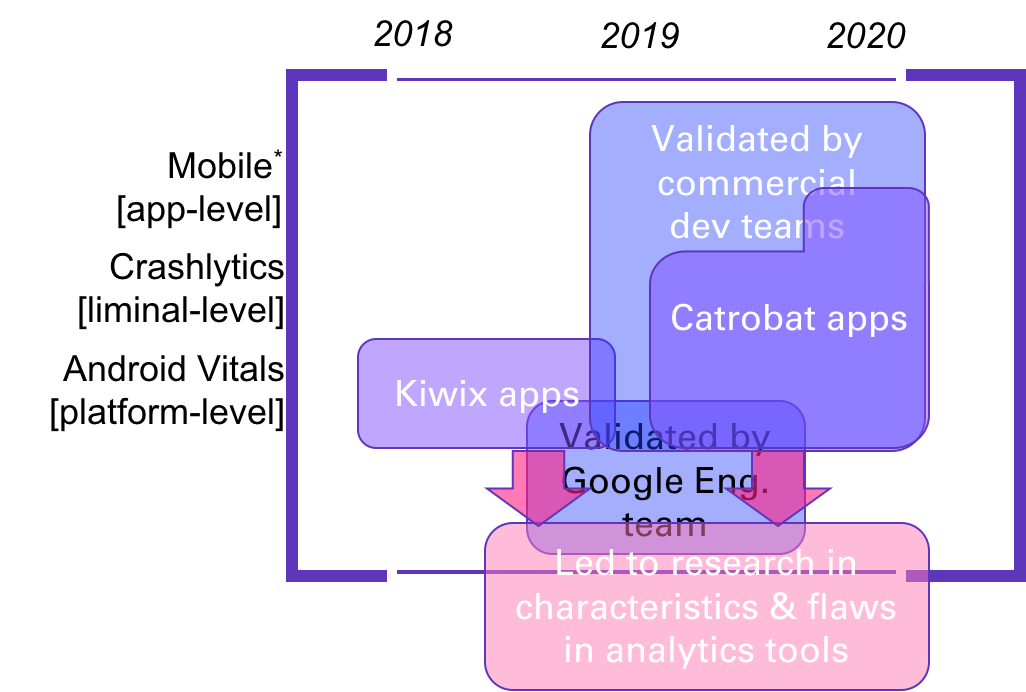
\includegraphics[width=10cm]{images/visual-connections-in-research.png}
    \caption{Visual Connections in my research}
    \label{fig:visual-connections-in-research}
\end{figure}

\textit{MUST-DO update this figure, it is out of date.} Figure \ref{fig:visual-connections-in-research}  aims to provide a visual overlay of the main practical elements of the research from 2018 to 2020. There are three main factors: 1) the type(s) of analytics used, 2) the development team and their apps, and 3) the progression of the case studies, as they augment what has been learned in earlier case studies.
% \akb{Why is it important to understand the timeline here - what implication does it have for understanding the research problem?}

The research started with the Kiwix~\footnote{The Kiwix project enables people to use Wikipedia and other content offline~\url{https://www.kiwix.org/en/}} set of Android apps where the app with the highest crash rate, as reported by Google's Android Vitals, was used as the experiment to see if the crash rate could be improved. By design the Kiwix apps do not include any analytics or crash reporting to minimise the digital usage footprint of these apps as they may be used in areas of the world where Wikipedia is banned, \emph{etc.} where the users may be persecuted or even imprisoned. Nonetheless, as the apps were available through Google Play (amongst many sources) the development team received ongoing reports in Google Play Console including the Android Vitals reports on various `stability' metrics as defined and applied by Google.

The Catrobat team was and is an extremely well researched and supported collection of mobile apps intended to help young people learn how to enjoy developing games visually. It was established % Removed details for the review period: "by Professor Wolfgang Slany of" 
at the TU Graz university where both undergraduate and postgraduate students actively practice software skills on the codebase. My engagement started around June 2019 and we jointly decided to pick the thornier and most complex Android app - Pocket Code - as the subject for our collaboration and research as it had proved to have an intractable ongoing issue with the high reported crash rate and therefore a worthy challenge for the concepts proposed in my research. We had a reference app, called Pocket Paint, which had a lower crash rate. Note: Pocket Paint was and is incorporated into Pocket Code in addition to being a standalone app.

Pocket Code already incorporated one of the most popular crash analytics library called Crashlytics. At the time, it used an older, mature version of Crashlytics branded Fabric (a business first acquired by Twitter, then by Google). I have chosen to use the term \emph{liminal}~\footnote{\url{https://www.lexico.com/en/definition/liminal}} to indicate crash reporting is something that lives in the boundary layer between the app and the operating system, or platform. Either is able to observe application crashes, and for apps where both the app and the platform capture information about crashes the two data sources can be usefully cross-referenced and compared, as my research has done.

As Pocket Code was an Android app, available in Google Play, the team also received the reports provided by Google through Google Play. These two data sources provided an interesting and rich set of research challenges. 

Relatively recently, in February 2020, the Catrobat team had to migrate their Crashlytics reporting from the Fabric service, which Google was ceasing, to Firebase the replacement reporting service Google provided. In parallel with this migration of the reporting the project team agreed to incorporate mobile analytics into their Android and iOS apps. They decided to use Firebase Analytics for various reasons (to be covered later in my thesis), hence the extension of the apps into app-level analytics.

The two arrows in the figure indicate an area of unplanned research: 
%
I discovered various flaws in the developer-oriented reports Google provides to app developers who make their apps available in Google Play (approximately 2.9 million apps globally). This led initially to discussions with the relevant engineering teams for Google Play and Android Vitals at Google where they confirmed various flaws. They asked for ongoing updates on my findings and requested a report which I provided. Through our interactions and discussions I realised the merit of researching the characteristics and flaws in analytics tools, and particularly those provided by Google for Android developers. This research is ongoing and intended to continue post PhD given the importance and relevance of the topic.

In mid-2019 several commercial Android development teams learned of my research and offered to contribute their experiences and practices of using mobile analytics in their commercial apps. These apps include app-level analytics in addition to the development teams receiving the ongoing reports Google provides automatically. The contributions of these development teams helped provide additional weight to the value and relevance of using mobile analytics to identify flaws in mobile apps and evidence of the importance developers placed on addressing quality issues gleaned through these tools.

%\yy{The practical research}{Need to complete the sentences, what is liminal? Change Kiwix/Catrobat apps to "Kiwix/Catrobat teams"? }

\begin{table}[htbp!]
    \centering
    \small
    \setlength{\tabcolsep}{4pt} %% default is 6pt
    \begin{tabular}{llrr}
      Case Study &Role of Researcher &Apps &Active Users\\
      \hline
       \href{https://play.google.com/store/apps/dev?id=9116215767541857492&hl=en_GB}{Kiwix}  &Embedded &18 &367K\\
       \href{https://play.google.com/store/apps/developer?id=Catrobat&hl=en_GB}{Catrobat} &Guide &6 &200K\\
       \href{https://play.google.com/store/apps/dev?id=7665838187257770408}{Greentech Apps} &Observed &10 &987K\\
       \href{https://play.google.com/store/apps/developer?id=Moonpig.com&hl=en_GB}{Moonpig.com} &Observed &1 &130K\\
       \href{https://play.google.com/store/apps/details?id=boundless.moodgym&hl=en_GB}{Moodspace app} &Interviewed &1 &20K\\
       \href{https://play.google.com/store/apps/details?id=com.localhalo.app&hl=en_GB}{Local Halo app} &Observed &1 &1.1K\\
       Commercial case study &Consultant &1 &1.9M\\
    \end{tabular}
    \caption{Project teams and Commercial apps in the case studies}
    \label{tab:case_studies}
\end{table}

For the Kiwix case study, the researcher has been an intrinsic long-term member of the diffuse project team, able to work directly with the code-base and collaborate directly with the developers and ancillary members of the project team. 

For the Catrobat case study, the researcher advised and assisted the project team to apply mobile analytics to their larger, older, and less reliable app: \emph{Pocket Code}. The researcher helped lead a one-day hackathon and otherwise interacted through a bug reporting tool, JIRA, discussions and using shared documents. Pocket Code also included a crash-reporting library which allowed cross-tool comparisons of reports, analytics and data. During the research, the reporting platform for the crash-reporting was migrated to a newer service which provided further insights and comparisons across and between the various mobile analytics tools.

The Greentech apps case study blends public and private sharing of their projects, they track issues in public, the codebase is private. Their active userbase is larger than the combined userbases of the Kiwix and Catrobat mobile apps. The team structure is similar to those for the Kiwix project, where it's a not-for-profit foundation where donations help fund some of the development work however many of the development team are part-time volunteers. Their core team are in Bangladesh, distant from the Western world and their focus is to enable native Bangla speakers to learn and study the Quran. Their priorities differ from those of most projects, the quality of their material is paramount and they sometimes disable support for apps that have serious quality flaws in these materials. 

For the commercial app teams (Moonpig, Moodspace, and LocalHalo), the researcher corresponded with one of the development team for each of the commercial apps and received either direct access to their analytics tools (LocalHalo), or was provided with snapshots (Moonpig and Moodspace). Permission was granted by their respective organisations for their contributions to be used for research purposes.

The corporate case study has an order of magnitude more complexity than the other apps with much higher demands on the software being reliable and performant. The business and the service provided through the client apps are expected to grow massively as the product matures and the software quality improves. While they include clients for MacOS, iOS, Android, webRTC, and Windows desktop operating systems, the case study focuses on the Android client.

How developers of Android apps actually use mobile analytics for remote logging compared to how developers use local logging focuses on the perceived purpose of the logging across over 100 opensource projects on GitHub.com. And the final case study is from the perspective of a startup who are developing and researching tools and techniques to help developers improve their design, implementation and use of usage analytics tools (both web and mobile apps). 
\newpage

\section{Kiwix Android Apps}
\label{section-kiwix-case-study}
\subsection{Introduction of Kiwix Android Case Study}
Relies solely on analytics and reports provided by the platform. We chose the most sophisticated and complex of the Android apps, which also had the highest Crash rate at the time. By applying what the team learned about crashes reported in Android Vitals the team was able to reduce the crash rate of this app several fold. When the improved codebase was used to refresh various custom apps their crash rates also decreased several fold.


\subsection{Case study of working with the Kiwix team}
As reported in \cite{harty_google_play_console_insightful_development_using_android_vitals_and_pre_launch_reports} and \cite{harty_better_android_apps_using_android_vitals} the Kiwix Android app had a very high overall crash rate caused by several significant flaws in the app. The project team released version 2.5 of the main Kiwix app in July 2019. As figure \ref{fig:kiwix_crash_rate_drops_v2_5} shows, the crash rate decreased significantly as version 2.5. In the last 30 days the crash rate was 1.87\% down from 5.07\% in February 2019.

One of the major changes in version 2.5 was the replacement of the in-house download utility with the default Android Download Manager\cite{kiwix_release_2_5_0}. The in-house version was a major source of crashes, and the replacement obviated a class of crashes, however it did so at a price in terms of functionality and usability. The in-house download utility allowed users to pause and resume downloads, and it would complete failed partial downloads. Users also received updates on the progress of the downloads, important when they often took many minutes or even hours or days in some cases (such as for multi-GB downloads over poor, slow, unreliable connections on low-end devices).

\begin{figure}[htbp!]
    \centering
    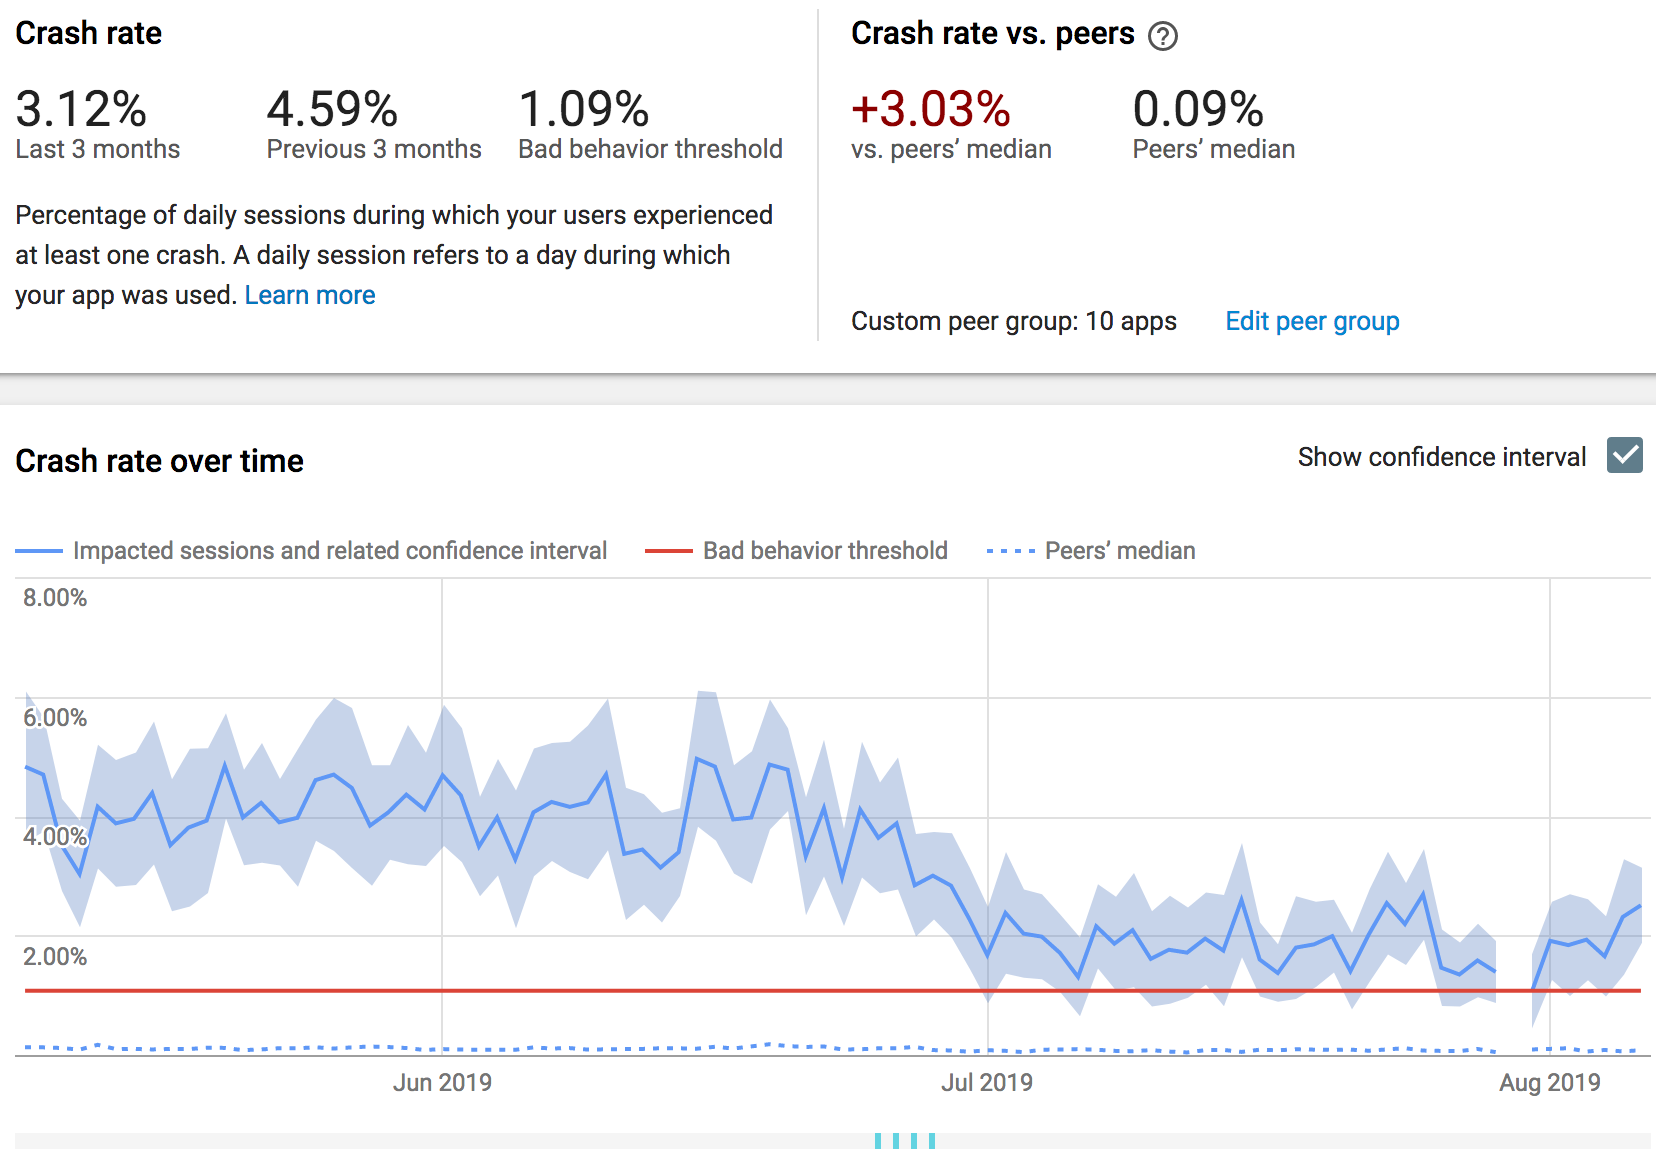
\includegraphics[width=\textwidth]{images/android-vitals-screenshots/kiwix-crash-rate-drops-with-v2_5.png}
    \caption{Kiwix Crash Rate Drops with V2.5 Release}
    \label{fig:kiwix_crash_rate_drops_v2_5}
\end{figure}

Following initial discussions about the crashes being reported in Android Vitals for version 2.5.0 of the Kiwix application, we collaborated on a week-long hackathon in Stockholm in August 2019. There, the developers ended up fixing some of the causes of the most frequent crashes with a surprisingly small amount of code of under 25 lines (including 10 lines of text added to the release log)\footnote{\url{https://github.com/kiwix/kiwix-android/pull/1388}}.

Several developers for the Kiwix project, the lead developer in particular, have been actively reviewing crashes reported by Android Vitals, filing issues, and addressing the causes of the crashes in order to reduce the crash rate and improve the app's stability. Evidence issues that mention crash: 133 closed, 6 open. \footnote{\url{https://github.com/kiwix/kiwix-android/issues?utf8=\%E2\%9C\%93&q=is\%3Aissue+crash}}
%TODO in a longer work, analyse each issue to identify the source of the crash.

Several releases later, each with various changes and improvements aimed at fixing causes of crashes the crash rate was materially lower than when we started, at the time of writing the overall crash rate for the last 7 days is 0.54\% which is inflated because the rash rate for the previous release (3.1.2) spiked at 1.38\%, compared to 0.18\% for release (3.0.5 -  the last production release) and 0.25\% for the recently released fix (3.1.3).

\subsection{Examples of real-time crashes}
Each of these examples exemplifies at least one characteristic of the reports that are provided by Android Vitals in Google Play.

\subsubsection{EsxRenderBucket::AddUnbucketedEntries(...)}
This crash is one of the most frequent crashes reported in early October 2020 and has been occurring on an ongoing basis according to Android Vitals for the current release of the Chemistry \& Physics simulations app (release 2020-04). Through analysis of the reports this crash only affects one release of the app (release 5200950) and it does not occur on the other three releases (6200950, 4200950, 3200950). It occurs on multiple manufacturer's device models, and on Android 9.0, 8.1, and 8.0). 

This crash is a native crash and mainly occurs within the context of \texttt{/system/app/Chrome/Chrome.apk} \textit{the web browser app created by Google!} The Kiwix apps rely on an embedded web browser, which is generally Google's Chrome browser, to render (\emph{i.e.} display) the content to the user\footnote{It also appears for other variants of the Android Chrome browser on some devices e.g. \texttt{/data/app/com.android.chrome-bAmCl9DcPfmqf3oKL54Efg==/base.apk (offset 0xbe7000)} and also the Android WebView component~\texttt{/data/app/com.google.android.webview-9ShSu\_81V02zu4ENrAjvJA==/lib/arm/libwebviewchromium.so} (also created by Google).}.

\begin{listing}[H]
\caption{Crash Cluster: EsxRenderBucket::AddUnbucketedEntries} \label{code:crash_cluster_add_unbucketed_entries}
\tiny
\begin{minted}{cpp}
*** *** *** *** *** *** *** *** *** *** *** *** *** *** *** ***
pid: 0, tid: 0 >>> org.kiwix.kiwixcustomphet <<<

backtrace:
  #00  pc 00000000001535a0  /vendor/lib/egl/libGLESv2_adreno.so (EsxRenderBucket::AddUnbucketedEntries(EsxCmdBufType, unsigned int)+132)
  #01  pc 0000000000152b17  /vendor/lib/egl/libGLESv2_adreno.so (EsxRenderBucket::BucketRenderingCmds(EsxRenderBucketParams*)+740)
  #02  pc 0000000000186a6d  /vendor/lib/egl/libGLESv2_adreno.so (EsxContext::BucketRenderingCmds(int)+712)
  #03  pc 00000000000e6987  /vendor/lib/egl/libGLESv2_adreno.so (EsxContext::BindDrawFramebuffer(EsxFramebufferObject*)+178)
  #04  pc 00000000000b6a5d  /vendor/lib/egl/libGLESv2_adreno.so (EsxContext::GlBindFramebuffer(unsigned int, unsigned int)+332)
  #05  pc 0000000001b8c659  /system/app/Chrome/Chrome.apk (offset 0x80c000)
\end{minted}

\end{listing}

Of the 53 crash clusters reported over the last 60 days for all Android versions and version 5200950 of the app, installed from Google Play, 16 of the 53 crash clusters are for this crash.

Searching local logs, generated using the opensource software~\texttt{vitals-scraper} that we created as part of this research we can see the same crash cluster has occurred in some, not all, of the Kiwix applications. The command used to find the files that contain this crash cluster is:~\texttt{grep -c EsxRenderBucket::AddUnbucketedEntries * | sort -t ':' -k 2 -g}. This returns a list of the files, sorted by the number of matches for the string found in each of the files. Here are the entries with at least one match.

\begin{listing}[H]
\caption{Logs that include crash cluster: EsxRenderBucket::AddUnbucketedEntries} \label{code:vitals_scraper_logs_add_unbucketed_entries}
\footnotesize
\begin{minted}{text}

android-crash-clusters-org.kiwix.kiwixcustomphet_1572958874833.json:2
android-crash-clusters-org.kiwix.kiwixmobile_1599898794048.json:2
phet-1-day-android-crash-clusters_1569599996989.json:2
android-crash-clusters-org.kiwix.kiwixcustomphet_1572966654935.json:3
android-crash-clusters-org.kiwix.kiwixmobile_1577913956806.json:3
android-crash-clusters-org.kiwix.kiwixcustomphet_1574380641173.json:4
android-crash-clusters-org.kiwix.kiwixcustomphet_1572976000060.json:5
android-crash-clusters-org.kiwix.kiwixcustomphet_1577913523667.json:5
android-crash-clusters-org.kiwix.kiwixcustomphet_1601883786819.json:5
wikimed-60-days-android-crash-clusters_1568705009571.json:6
phet-7-days-android-crash-clusters_1569484818005.json:13
android-crash-clusters-org.kiwix.kiwixcustomphet_1573403158401.json:14
android-crash-clusters-org.kiwix.kiwixcustomphet_1599898464809.json:14
phet-60-days-android-crash-clusters_1568703927627.json:18
android-crash-clusters-org.kiwix.kiwixcustomphet_1572903426940.json:21
phet-60-days-android-crash-clusters_1565933377493.json:21
android-crash-clusters-org.kiwix.kiwixcustomphet_1572812538185.json:25
\end{minted}

\end{listing}

From these results the crash occurs most often in the Physics \& Chemistry simulation custom app (these include the phrase `phet'\footnote{`phet' is the term used for the source of the contents used in this custom app, i.e. the source of the various Chemistry and Physics simulations, written in HTML5. They are extremely rich in terms of their content and dynamic rendering as they provide interactive, dynamic simulations.} as part of the filename. It also occurred relatively infrequently in two other of the apps: five times in the core Kiwix app, and six times in the Wikipedia in English app. The core Kiwix app can be used with the same contents as the project bundles in the custom apps, so some of the crashes~\emph{might} be for the same content, we don't know enough from the stack trace to determine the contents. the reasons for the error in the custom WikiMed app are not known at this stage. 

Searching online, using Google Search, for \texttt{EsxRenderBucket::AddUnbucketedEntries} finds a similar stack trace occurs with the Unity SDK and it appears to be related to a particular chipset:
\begin{itemize}
    \item \href{https://developer.qualcomm.com/forum/qdn-forums/software/adreno-gpu-sdk/67924}{Forums - Help with crash in {\footnotesize libGLESv2\_adreno.so (EsxRenderBucket::AddUnbucketedEntries)}} 2020
    % \item \href{https://github.com/flutter/flutter/issues/38676}{/system/vendor/lib/egl/libGLESv2_adreno.so #38676} 2019
    % \item \href{https://stackoverflow.com/questions/29728931/libglesv2-adreno-so-game-crash-in-galaxy-note-4-and-lollipop-5-0}{libGLESv2_adreno.so game crash in Galaxy Note 4 and Lollipop 5.0} 2015
    \item \href{https://forum.unity.com/threads/unity-2019-android-build-crashes-on-devices-using-adreno-506-gpu.712229/}{Unity 2019 Android build crashes on devices using Adreno 506 GPU}. This bug report includes several different method names where the crash occurs. Various developers report the issue, \href{https://forum.unity.com/members/waldgeist.1371619/}{Waldgeist} reporting the one with this method name.
\end{itemize}

The bug appears hard for developers to reproduce and from the app developer's perspective it happens in software they cannot fix themselves. 

As Ogien reports in~\href{https://forum.unity.com/threads/unity-2017-2-crashes-vs-5-6-2f1.511995/}{Unity 2017.2 Crashes vs 5.6.2f1} they may be able to identify correlations (in this example using a screenshot from Android Vitals, I believe, as shown in Figure~\ref{fig:unity-2017-2-android-vitals-annotated-graph}). The Unity support team state the bug may have been fixed and the developer promised to try the new release and report back at the time, in 2018, however they have not done so online at least\footnote{This user was online more recently, including \nth{24} September 2020.} so that issue has an indeterminate result from a research perspective.

\begin{figure}[htbp!]
    \centering
    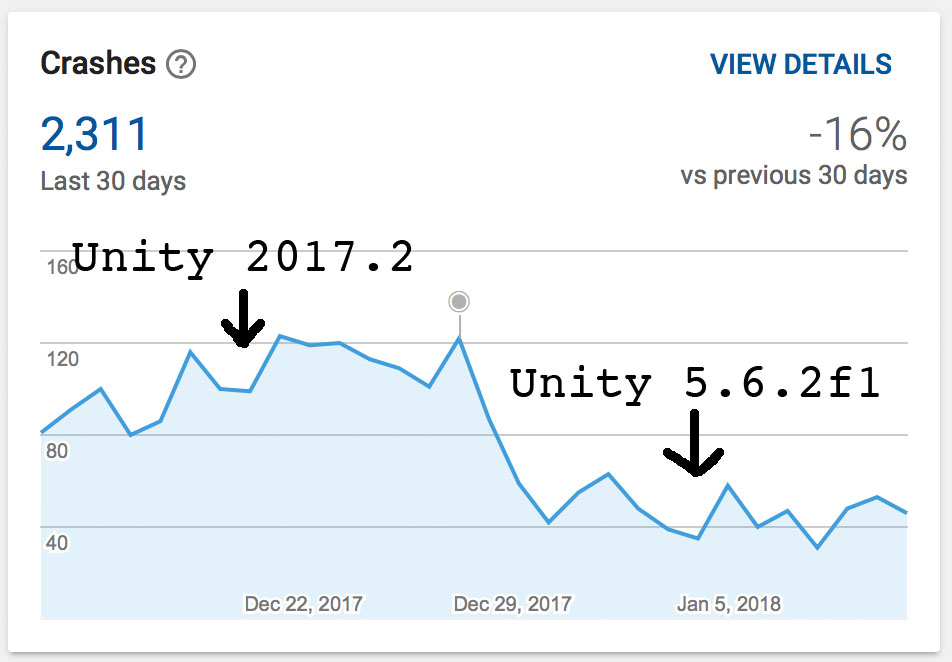
\includegraphics[width=12cm]{images/unity-forum/unity-2017-2-android-vitals.jpg}
    \caption{Unity 2017.2 Android-Vitals annotated graph (\url{https://forum.unity.com/threads/unity-2017-2-crashes-vs-5-6-2f1.511995/}}
    \label{fig:unity-2017-2-android-vitals-annotated-graph}
\end{figure}

MUST-DO Discuss the augmented crash stack trace utility, how it works, and why we did~\emph{not} use it in Google Play apps.


\subsection{Lessons learned from this case study}

As~\citep{kidwell2015_toward_fault_taxonomy_application_of_software_analytics} notes, previous research by~\citep{weider1998_software_fault_prevention_in_coding_and_RCA} nearly half the faults were introduced during coding and \emph{``...many of the faults were preventable"}. These results were borne out in the Kiwix Android case study where some of the most frequent crashes were null pointer errors in the Java code. For the Kiwix Android project one of the longer term challenges was the youth of many of the volunteer contributors including some of the development leads who were often teenagers and pre-undergraduate level software developers who wouldn't have the expertise expected of professional software developers\footnote{(They often joined via Google Code-in~\citep{google_code_in_archive} or Google Summer of Code~\citep{google_summer_of_code}).}. While there may well be training techniques and software tools, including Android Lint, that may have been able to find some of the causes of the crashes reported by Android Vitals it's unlikely that these volunteers would choose to use those tools or want to undergo training. And as interviews with developers demonstrated the perceived effort of dealing with static analysis reports and the volume of false positives mean developers don't use static analysis tools very often to find bugs~\citep{johnson2013_why_dont_devs_use_static_analysis}.

\subsection{Summary of Kiwix Android Case Study}
TBC
\newpage

\section{Catrobat Android Apps}
\subsection{Introduction to the Catrobat Case Study}
This case study includes an extremely and unusually well researched and properly developed app and codebase where many of the perceived good practices were and are assiduously applied on an ongoing basis. The codebase is far more complex than the Kiwix Android apps and the app is significantly richer in terms of the features and functionality.

This case-study includes some in-app analytics, in the form of a crash reporting tool called Crashlytics. This additional source of analytics identified additional concerns with analytics tools as the two sources of analytics (Google Play Console and Crashlytics) had significant differences in their calculations and reports. It illustrates the efficacy of investigating crashes reported by the analytics where relatively minor effort was needed to identify and fix causes of poor reliability.

Furthermore, the project team chose to invest their energies into supporting a testing workshop in Poland and to introducing application-level in-app analytics to both their Android and iOS PocketCode apps. Their actions indicate the project team recognise the benefits of applying and incorporating analytics into their software development and quality improvement practices.

\subsection{Potted History of the Project}
\begin{enumerate}
    \item Rationale:
    \item Involvement of under-grads and post-grads. Master's theses (ask for stats).
    \item External contributors: translations, rich community contributions of PocketCode apps, ...
    \item Catrobat foundation, and funded work.
    \item Software Development, testing, maintenance,...
\end{enumerate}
Rationale,
Involvement of under-grads and post-grads. Master's theses (ask for stats)
Catrobat foundation, and funded work.

\subsubsection{Catrobat Software Engineering Practices}
Approach to development, testing, deployment, production monitoring, ...

The project uses Jenkins to run continuous builds for PocketCode and other related projects \url{https://jenkins.catrob.at/job/Catroid/}. Most of the builds are for the Develop code branch \url{https://jenkins.catrob.at/job/Catroid/job/develop/}.

At the start of the case study the crash rate of the Pocket Code app remained stubbornly high despite the extensive use of code quality tools and practices, automated testing, continuous builds and so on. In the product view of quality, ~\citep{kitchenham1996_software_quality_elusive_target}, observed that the approach of taking a product view of quality~\emph{``is frequently adoptd by software-metrics advocates, who assume that measuring and controlling internal product properties (internal quality indicators) will result in improved external product behavior (quality in use)."}~\footnote{US English spelling was used in the original article so used here in the quotation.} Back when the article was published, in 1996, the authors stated \emph{``more research was needed to determine which aspects of internal quality affect the product's use."}

\subsection{Method}
Discussions, co-organised a hackathon in Graz, Austria at the project's parent university, planned for 24 hours from 9am 16th November 2019. 

Hackathon focus: to improve code quality based on failures and issues reported in Android Vitals (cross-referenced with those reported in Fabric Crashlytics).

\subsection{The Project's Working Practices}
Specific roles, who can do what.
Issues need to be reported in JIRA in order for any code to be considered

\subsection{Introduce the Analytics Tools}
\begin{enumerate}
    \item Types of crashes: Soft crashes (mapping terminology between Fabric Crashlytics and Android Vitals).
\end{enumerate}

\subsection{Summary of the Hackathon}
The visit (including the presentation at the Graz University of Technology on Friday morning and to Dynatrace\footnote{\url{https://www.dynatrace.com}} on Friday afternoon) helped reinforce the value of creating and using the Vitals-Scraper software to preserve history. 

How many participated (including Wolfgang and Matthias in non-coding capacities). Approximate time spent. Twenty-two (22) issues were raised during the day (tagged: hackathon-2019)\footnote{\url{https://jira.catrob.at/browse/CATROID-426?jql=labels\%20\%3D\%20hackathon-2019}}. Most of these were created in the morning, one for each of the top crashes and ANRs as recorded and ranked in Android Vitals. 

\subsection{Results}
We can group the issues using as follows (already fixed, addressed during the hackathon, pending, rejected).

\subsubsection{Already fixed} JIRA issue 405\footnote{\url{https://jira.catrob.at/browse/CATROID-405}} was the \#1 issue with over 2000 crashes reported in the 30 days preceding the hackathon (and over 3200 in the lifetime of the app). However, it had already been addressed in JIRA issue 379\footnote{"media download progress dialog crashers" \url{https://jira.catrob.at/browse/CATROID-379}} and incorporated in to the most recent release \footnote{Release:
0.9.65 Nov 13, 6:01 PM: Full rollout.} as part of a major effort to improve the code quality around the embedded WebView component.

Early indications are that the fixes related to the WebView have made a material improvement in the crash-rate for PocketCode 2.45\% vs. 3.9.3\% on Monday \nth{18} November 2019; details are in Table \ref{tab:androidvitals_rollout_of_0_9_65}. Therefore, in terms of assessing any improvement that results from the work of the hackathon the baseline is 2.45\%.

% TODO perhaps move these to a Glossary section?
% Number of sessions tool-tip: Approximate number of recorded sessions
% Crash-free sessions tool-tip: Percentage of daily sessions during which your users did not experience any crashes. A daily session refers to a day during which your app was used.
% Impacted sessions tool-tip: Percentage of daily sessions during which your users experienced at least one crash. A daily session refers to a day during which your app was used.
\begin{table}[ht]
    \centering
    \footnotesize
    \begin{tabular}{r|r|r|r}
        App version &Impacted sessions &Crash-free sessions &Number of sessions  \\
        \hline
        69 (0.9.65) &2.45\% &	97.55\% 	&~800 \\
        Production &&& \\
        \hline
        66 (0.9.64) &3.93\% &96.07\% 	&~3K
    \end{tabular}
    \caption{AndroidVitals: Improvement in crash-rate post WebView improvements}
    \label{tab:androidvitals_rollout_of_0_9_65}
\end{table}

The change was to remove a progress dialog for media downloads. The development team was not able to reproduce the crash according to the JIRA ticket or the code review in the pull request \#3362\footnote{\url{https://github.com/Catrobat/Catroid/pull/3362/files}}. And yet the fix seems to have had the desired effect in terms of the crash rate. The effect on the UX is not known.

\subsubsection{Addressed During the Hackathon}
Some of the issues were determined to be 'soft errors' that were leaking to Android Vitals even though the app handled / recovered from them. These were addressed through the work recorded in  \href{https://jira.catrob.at/browse/CATROID-426}{CATROBAT-426}. Table \ref{tab:hackathon_2019_jira_addressed} provides a brief summary of all the issues addressed in the hackathon.


\href{https://jira.catrob.at/browse/CATROID-418}{CATROID-418 - Crash in PlaySoundAndWaitBrick.addActionToSequence} The author paired with one of the developers on this issue. It is believed to be a bug that can only occur at runtime when the user has deleted the sound file that is being used by the \texttt{PlaySoundAndWaitBrick} which raised an \texttt{IllegalArgumentException} as it cannot determine the path from the Java Object that represented the sound file for this PocketCode visual programming element. We were able to reproduce the error on a local device and implement a fix. The developer thought a similar behaviour might be the cause of the exception reported in issue \href{https://jira.catrob.at/browse/CATROID-419}{419}, this has yet to be investigated.

\begin{table}[ht]
    \footnotesize
    \centering
    \begin{tabular}{rll}
        JIRA Ticket &Category &Remarks \\
        \hline
        \href{https://jira.catrob.at/browse/CATROID-407}{CATROBAT-407} &NullPointerException &Soft error already handled by app. \\
        \href{https://jira.catrob.at/browse/CATROID-409}{CATROID-409} &NullPointerException &Crash in showLegoSensorConfigInfo
        \\
        \href{https://jira.catrob.at/browse/CATROID-418}{CATROID-418} &IllegalArgumentException &Crash in \\&&  PlaySoundAndWaitBrick.addActionToSequence \\
        %SHOULD_DO fix Temporary hack to wrap above text.

    \end{tabular}
    \caption{Hackathon bugs addressed during hackathon.}
    \label{tab:hackathon_2019_jira_addressed}
\end{table}

\subsubsection{Pending} 
Table \ref{tab:hackathon_2019_jira_issues_pool} summarises the issues that were raised and were not actioned during the hackathon.

Of these, \href{CATROID-410}{https://jira.catrob.at/browse/CATROID-410} and \href{https://jira.catrob.at/browse/CATROID-412}{CATROID-412}seem, as issue \href{CATROID-405}{https://jira.catrob.at/browse/CATROID-405} was, to have been fixed in the recent release 0.9.65 (69). Android Vitals shows these crashes last occurred in the previous release of 0.9.64 (66).

Similarly, issues \href{https://jira.catrob.at/browse/CATROID-413}{CATROID-413 - Crash in saveScreenshot} has not yet been reported for the current release: 0.9.65 (69).

\href{CATROID-411}{https://jira.catrob.at/browse/CATROID-411} is for an ANR (where the app freezes) when taking a screenshot. This occurs in both the previous and current releases and is currently being investigated by one of the development team.

\href{https://jira.catrob.at/browse/CATROID-413}{CATROID-413 - Crash in LineTool.draw} seems to be a long-running issue, found in releases (65), (66), and the current release (69).

\href{https://jira.catrob.at/browse/CATROID-415}{CATROID-415 - Crash in onBackPressed} is another long-running release however it is happening much more often - twenty-eight times by Monday \nth{18} November 2019 in the current release (69), versus once in release 63 (on \nth{23} October 2019. Of the crashes in (69) happened on the same day as the hackathon - perhaps the participants were triggering albeit they might not be aware of it? If they weren't aware, this might be another instance where the issue is a 'soft-error' which is handled by the app and therefore suitable for similar treatment to that proposed in \href{https://jira.catrob.at/browse/CATROID-426}{CATROID-426}?

\href{https://jira.catrob.at/browse/CATROID-416}{CATROID-416 - Crash in VisualPlacementActivity} from Android Vitals, this crash has only been reported in the current release 0.9.65 (69). It affected a range of devices and occurred on at least 2 Android versions.

\href{https://jira.catrob.at/browse/CATROID-417}{CATROID-417 - Crash in MainMenu onCreate} may be newly introduced in 0.9.65 (69). This has only been reported for a single user who experienced it 4 times. The exception is a \texttt{java.lang.ClassCastException} perhaps it's triggered by a particular PocketCode script or method call?

\href{https://jira.catrob.at/browse/CATROID-420}{CATROID-420 - Crash in resolveFileName} This was addressed two days after the hackathon and merged into the next release 0.9.66 (70). The crash was newly reported in 0.9.65 (69) and happened twice, once on an Huawei Y9 and once on an Honor 7X.

\href{https://jira.catrob.at/browse/CATROID-421}{CATROID-421 - ANR in MainMenuActivity} This ANR was reported in both 0.9.64 (66) and 0.9.65 (69) and has been reported on Android 7.0 and 7.1 on 3 distinct device models with all bar one on Xiaomi devices, the remaining crash is on a Lenovo VIBE K6 Note (K53a48), with Android 7.0.

\href{https://jira.catrob.at/browse/CATROID-423}{CATROID-423 - ANR in ProjectActivity} This ANR has also occurred in the most recent release: 0.9.66 (70). It's been reported 7 times on 4 device models in the last 30 days and on both Android 7.0 and 7.1

From the trace, perhaps it's related to taking a screenshot? Also, the queue delay can be over 18 seconds - far longer than anyone would like:

\texttt{\small{"Input dispatching timed out (org.catrobat.catroid/org.catrobat.catroid.ui.ProjectActivity, Waiting to send non-key event because the touched window has not finished processing certain input events that were delivered to it over 500.0ms ago. Wait queue length: 28. Wait queue head age: 18726.7ms.)"}}

\href{https://jira.catrob.at/browse/CATROID-424}{CATROID-424 - ANR in SpriteActivity} This ANR is also reported in newer 0.9.66 (70) and older releases, see \ref{tab:catroid_424}:
\begin{table}[ht]
    \centering
    \begin{tabular}{r|r|r}
Release	&Instances	&Percent \\
\hline
66	&12	&63.2\% \\
69	&6	&31.6\% \\
70	&1	&5.3\% \\
    \end{tabular}
    \caption{By app version for CATROID-424 issue}
    \label{tab:catroid_424}
\end{table}

The error summary is:
\texttt{\small{
Input dispatching timed out (AppWindowToken{c8e9f token=Token{b3ee03e ActivityRecord{4ed08f9 u0 org.catrobat.catroid/.ui.SpriteActivity t12205}}}, Waiting because no window has focus but there is a focused application that may eventually add a window when it finishes starting up.)}}

\href{https://jira.catrob.at/browse/CATROID-425}{CATROID-425 - tgkill crashes} There are various crash clusters for \texttt{tgkill}, 19 in 60 days to \nth{1} December 2019 across all versions of the app and Android versions. These have not been investigated yet. The ticket includes references to various guides to help investigate the causes.

\begin{table}[ht]
    \centering
    \footnotesize
    \begin{tabular}{r|l|l}
        JIRA Ticket &Category &Remarks \\
        \hline
        \href{https://jira.catrob.at/browse/CATROID-406}{CATROBAT-406} &NullPointerException &...BrickBaseType.getDragAndDropTargetList. \\
        \href{https://jira.catrob.at/browse/CATROID-408}{CATROID-408} &NullPointerException &Crash in Save Project. \\
        \href{https://jira.catrob.at/browse/CATROID-410}{CATROID-410} &NullPointerException &Crash in saveLegoNXTSettingsToProject \\
        \href{https://jira.catrob.at/browse/CATROID-411}{CATROID-411} &ANR &\texttt{StageListener.takeScreenshot} \\
        \href{https://jira.catrob.at/browse/CATROID-412}{CATROID-412} &NullPointerException &Crash in SetBackgroundEventId.hashCode \\
        \href{https://jira.catrob.at/browse/CATROID-413}{CATROID-413} &NullPointerException &Crash in saveScreenshot \\
        \href{https://jira.catrob.at/browse/CATROID-414}{CATROID-414} &NullPointerException  &Crash in LineTool.draw \\
        \href{https://jira.catrob.at/browse/CATROID-416}{CATROID-416} &NullPointerException &Crash in VisualPlacementActivity \\
        \href{https://jira.catrob.at/browse/CATROID-417}{CATROID-417} &ClassCastException &Crash in MainMenu onCreate \\
        \href{https://jira.catrob.at/browse/CATROID-420}{CATROID-420} &SecurityException &Crash in resolveFileName \\
        \href{https://jira.catrob.at/browse/CATROID-421}{CATROID-421} &ANR &MainMenuActivity \\
        \href{https://jira.catrob.at/browse/CATROID-423}{CATROID-423} &ANR &ProjectActivity \\
        \href{https://jira.catrob.at/browse/CATROID-424}{CATROID-424} & ANR &SpriteActivity \\
        \href{https://jira.catrob.at/browse/CATROID-425}{CATROID-425} &tgkill &Various crash clusters \\
    \end{tabular}
    \caption{Hackathon bugs in the "Issues Pool"}
    \label{tab:hackathon_2019_jira_issues_pool}
\end{table}

\subsubsection{Rejected}
\href{https://jira.catrob.at/browse/CATROID-422}{CATROID-422 - Crash at org.catrobat.catroid.ui.ProjectActivity.showLegoSensorConfigInfo } \texttt{(ProjectActivity.java:396)} %TODO work out why I needed to split the above to avoid a latex compile error.
This was rejected by one of the developers as they wanted to suppress the crash (which is considered one the app recovers from) through \href{https://jira.catrob.at/browse/CATROID-426}{CATROID-426}. Interestingly the 'fix' did not stop this crash from being reported in 0.9.66 (70).

\subsubsection{Permission Denials}
One of the Android Vitals "qualities" pertains to how often users deny permissions requested by an app. A low percentage (ideally zero) is their target recommendation. As Table \ref{tab:pocketcode_permission_denials} shows, PocketCode has a significant percentage of denials, 4.74\% as of \nth{18} November 2019. In discussion with the project lead, Prof. Wolfgang Slany, during the hackathon, this is a known consideration. The project team aims to improve the behaviour (\emph{i.e.} the design and implementation). The app currently asks users early on for permission to check the memory card in order to find PocketCode projects. As the permission dialog asks about access to read photos and videos, etc.\todo{Add screenshot and correct wording} it does not seem relevant to some users and they say no. As others have determined\todo{add references to design and timing of when to ask users things}  when and how an app asks a user has affects the outcomes.

% The following was copy-pasted from Android Vitals on 18th Nov 2019 for the PocketCode app.
% Metric 	Last 30 days 	Previous 30 days vs. peers’ median The difference between you and the peers’ median
% Permission denials Percentage of daily permission sessions during which users denied permissions. A daily permission session refers to a day during which your app requested at least 1 permission from its user. If a user makes multiple decisions for the same permission, only the final decision at the end of a day is recorded. Transparently explaining the reasons for permission requests can help reduce permission denials. 	4.74% 	4.39% 	-

% https://play.google.com/apps/publish/?account=8841632091579025670#AppHealthDetailsPlace:p=org.catrobat.catroid&appid=4975762901432177859&aho=APP_HEALTH_OVERVIEW&ahdt=PERMISSION_DENIAL&ts=THIRTY_DAYS&ahbt=_APPLICATION

\begin{table}[ht]
  \centering
    \begin{tabular}{lrrr}
        Metric 	&Last 30 days\footnote{As of \nth{18} Nov 2019} 	&Previous 30 days &vs. peers’ median  \\
        Permission denials\footnote{Percentage of daily permission sessions during which users denied permissions. A daily permission session refers to a day during which your app requested at least 1 permission from its user. If a user makes multiple decisions for the same permission, only the final decision at the end of a day is recorded. Transparently explaining the reasons for permission requests can help reduce permission denials.} & 4.74\% 	&4.39\% 	&- \\

    \end{tabular}
    \caption{AndroidVitals: PocketCode: "Permission Denials"} 
    \label{tab:pocketcode_permission_denials}
\end{table}
% MUST-DO replace with threeparttable or similar. See https://tex.stackexchange.com/questions/108584/how-best-to-change-the-font-size-etc-of-threeparttables-table-notes/495973#495973

% Thanks to 
% https://stackoverflow.com/questions/2888817/footnotes-for-tables-in-latex#2891556
% TODO investigate suggestions from https://texblog.org/2012/02/03/using-footnote-in-a-table/ which look like they'll help improve the formatting of the table while also supporting footnotes.

\subsubsection{1 Week on}
Release 0.9.65 is now the dominant release, with ~4000 sessions between \nth{17} and \nth{23} November, compared to ~600 sessions for the previous release of the app (0.9.64). The overall reported crash rate reduced to 2.10\% for \nth{18} to \nth{23} November, compared to the previous 7 days crash rate of 3.62\%. \textbf{Note these are for releases that predates the hackathon.}

During a call with Professor Slany on \nth{25} November, he mentioned they had planned to release a new version of the app on Friday to address the loss of Fabric Crashlytics data and several improvement related to the hackathon; however their Jenkins build was coincidentally broken that day \url{https://jenkins.catrob.at/job/Catroid/job/develop/1098/} where the build failed to complete for over 54 hours. The cause was being investigated. According to logs on Jenkins it may be related to Docker not being available \texttt{Cannot connect to the Docker daemon at unix:///var/run/docker.sock. Is the docker daemon running?} \footnote{\url{https://jenkins.catrob.at/view/Catroid/job/Catroid/job/develop/1102/execution/node/27/log/}}

\subsubsection{2 weeks on}
\nth{1} December 2019.

A new release of the app was launched on November \nth{26} after several days of problems with the Jenkins CI pipelines which delayed this release by about 4 to 5 days.

The new release 0.9.66 (70) seems to have made a slight improvement to the overall crash rate which is currently 1.95\% after 3 days of data in Android Vitals, the previous release has a crash rate of 2.56\% for the last 7 days (to \nth{29} November. It is premature to determine the overall effect of the crash rate for this app as it's still being rolled-out (which typically takes over a week to reach the majority of the user-base e.g. on \nth{2} December (4 days after the release started rolling out) Android Vitals reports 20K install events).

The ANR rate is also showing encouraging signs, for the last 7 days (actually it seems to be only for 6 days, from \nth{24} to \nth{29} November 2019 as reported on \nth{1} December 2019) in Table~\ref{tab:ANR_rate_24_to_29_Nov_2019}.

\begin{table}[ht]
    \centering
    \footnotesize
    \begin{tabular}{r|r|r|r}
      App version  &Impacted sessions &ANR-free sessions &No. sessions \\
      \hline
      70 (0.9.66) Production &0.30\% &99.70\%	&~700 \\
      69 (0.9.65)            &0.46\% &99.54\%	&~3K  \\
    \end{tabular}
    \caption{PocketCode: ANR rate for Last 7 days}
    \label{tab:ANR_rate_24_to_29_Nov_2019}
\end{table}

\subsection{Progress in cumulative releases}

% MUST_DO add screenshots and summaries of the progress made with subsequent releases of Pocket Code for Android.


\subsection{Discussion}
Effects of being measured is a well-known in work, business, etc. One of the effects here was that 'soft-crashes' were reaching Android Vitals and therefore significantly and adversely affecting the crash rate (see \cite{CATDROID-426-JIRA}).

\subsubsection{Peer Groups}
The Pocket Code Android app had a significantly higher crash-rate compared to its peer group, as Figure \ref{fig:pocketcode_peer_crash_rate_18_nov_2019} shows in section \href{android-vitals-peer-groups}{\emph{\nameref{android-vitals-peer-groups}}} shows. While this may be undesirable, the Pocket Code app had incredible richness and complexity compared to the perceived peer apps, for instance it includes support for generating native Android apps, an app store, generation of rich, graphical games, as examples of some of the rich capabilities on offer.


\subsubsection{Slower growth of user-base}
PocketCode is an app developed to serve several challenges simultaneously, including research aspects such as the effects of various software development engineering practices, while also being intended to be open, in terms of informing the end-user of the purposes of the app, yet also being easy, fun and educational for children to use in terms of exploring how to write and publish software. These various concurrent challenges led to the users being presented with a long page of legal text (reformatted slightly from the original \href{https://github.com/Catrobat/Catroid/blob/develop/catroid/src/main/res/values/strings.xml}{\textbf{\texttt{Privacy policy on GitHub}}} and reproduced below in Listing~\ref{pocketcode-privacypolicy}). New users are expected to read and agree to before they are allowed to use the app further. Imagine having to scroll through all the text on a small screen \emph{before seeing what the app can do!} The thesis continues after the listing...

% COULD_DO there's lots of scope to tidy up this listing at some point.

\definecolor{dkgreen}{rgb}{0,0.6,0}
\definecolor{gray}{rgb}{0.5,0.5,0.5}
\definecolor{mauve}{rgb}{0.58,0,0.82}

\lstset{frame=tb,
  language=Cobol,
  aboveskip=3mm,
  belowskip=3mm,
  showstringspaces=false,
  columns=flexible,
  basicstyle={\tiny\ttfamily},
  numbers=left,
  numberstyle=\tiny\color{gray},
  %keywordstyle=\color{blue},
  commentstyle=\color{dkgreen},
  %stringstyle=\color{mauve},
  breaklines=true,
  breakatwhitespace=true,
  tabsize=2
}
\begin{multicols}{3}
% \lstinputlisting[{language=[LaTeX]TeX},breaklines=true]{\jobname.tex}

\begin{lstlisting}[caption={Privacy Policy for Pocket Code},captionpos=b,label={pocketcode-privacypolicy}]
Welcome!
Before you can start coding, please read and accept our Privacy Policy to use the app:
To offer you all the benefits of our services and the associated account, it is necessary to collect certain data from you.
* To maintain and improve our services (apps and websites) and to do scientific research on ICT and STEM/STEAM education, we use Google Analytics, Crashlytics, and Firebase, all by Google LLC (USA), as well as Dynatrace by Dynatrace LLC (USA) to get metadata about the usage of our services, e.g., crash information, timestamps, visited pages/screens, usage of our apps and services, used operating system, and information about the network provider. This analysis and the collected data is not linked to your profile and does not contain any personal information (last bits of the IP address get anonymized). However, the collected data will get transferred to the service-provider (Google LLC, USA and Dynatrace LLC, USA). 
Data processing is based on agreements with Google LLC and Dynatrace LLC. 
This relationship to the service provider conforms to the European Union\'s General Data Protection Regulation (EU GDPR) and EU-USA \"Privacy Shield\" agreement.
* To create and use an account in our systems, and to inform you about necessary changes about your account per e-mail, e.g., updates or violations of our Terms of Use and Service, our community rules, or our policies, we will store your username and, if provided by you, your e-mail address. If you have connected your account via your Google or Facebook account, we additionally store an identification key connected to your account on these services. We will not use this data for any other (e.g., marketing) purposes, unless you explicitly allowed us to do so.
* On a voluntary basis, you can give us your country of residence through your account page on the sharing site. This will get displayed on your public profile and only be used for statistical and research purposes by us. It can be removed at any time in your profile settings.
* You can withdraw the usage of the personal data belonging to your account at any time by deleting your account through your profile page on https://share.catrob.at. After deleting your account you will still be able to use the provided services, but not to collaborate, e.g., through uploading programs, commenting, or liking. Also, all provided content linked to your account, e.g., uploaded programs, comments, etc., will be deleted.
* To avoid misuse of our services, e.g., through user contributed uploads or comments for illegal purposes, all user generated public data (uploads, comments) will be stored internally in a database, together with a timestamp and the used internet address. This data will not be used by or forwarded to any institutions, unless sufficiently illegal actions are reasonably suspected and officially entitled legal institutions request it based on applicable law. Each case will be thoroughly checked on an individual basis by us first.
* You can voluntarily subscribe to the Catrobat Newsletter, on https://catrob.at/newsletter provided by us through the MailChimp service (The Rocket Science Group LLC d/b/a MailChimp, USA). You will then receive updates on the Catrobat project and its services to your provided e-mail address. You can withdraw the newsletter at any time by using the \"unsubscribe\" link in the footer of every newsletter. This newsletter is provided by MailChimp with whom we do have a data-processing agreement and who committed to the EU General Data Protection Regulation and EU-USA \"Privacy Shield\". For further details on MailChimp please also look up MailChimp\'s Privacy Policy and Terms of Use.
* All Services are provided by the free open source Catrobat project under the umbrella of the International Catrobat Association - Verein zur Foerderung freier Software, a non-profit NGO incorporated in Graz, Austria (European Union). Our policies pay respect to EU and Austrian data protection law (GDPR). To get in touch with us, please send an e-mail to contact@catrobat.org or mail us to Catrobat,
    c/o
    Institute of Software Technology,
    Graz University of Technology,
    Inffeldgasse 16b,
    A-8010 Graz, Austria
    (European Union).
In case you are below the age of 14, this policy must be accepted by a legal guardian (usually a parent).

Catrobat\'s official English language privacy policy is available on the web under https://catrob.at/privacypolicy.

Version 2.2, 17 October 2019

Find the previous, outdated, version of our privacy policy (2.0) here: http://developer.catrobat.org/privacy_policy_2-0
\end{lstlisting}
\end{multicols}
% Inspired by https://tex.stackexchange.com/questions/34098/two-column-code-listings-in-appendix-in-a-one-column-report

Welcome back. 

I hope the experience of scrolling past the privacy policy here provided you with an idea of how adding a mandatory, relatively comprehensive privacy policy interrupts the flow. One of the topics in the future work chapter, \href{enhancing-quality-vs-enhancing-ux}{\textit{\nameref{enhancing-quality-vs-enhancing-ux}}}, considers whether developers may obtain greater return on their investment by improving user experience rather than improving technical qualities of an app. As \href{enhancing-quality-vs-enhancing-ux}{Figure \ref{fig:Firebase-pocketcode-android-7-day-new-user-retention-29-may-2020}} shows, the Pocket Code app only retains 4\% of new users by day 2. Perhaps, the low retention rate may restrict the growth of the user-base even though the quality has improved markedly.

\subsubsection{Catrobat iOS Pocket Code App}
A more recent codebase, aimed at providing similar functionality to the Android Pocket Code app. This codebase is written specifically for iOS using the mainstream iOS development tools and development environment. 

In February 2020 the development lead for the iOS app, in conjunction with me and the overall project lead, Professor Wolfgang Slany, decided to add Firebase Analytics to the iOS codebase and implement crash reporting and in-app analytics. 

\begin{itemize}
    \item The design document
    \item The implementation process and effort needed
    \item Early discoveries (discussed at the workshop in Poland on \nth{28} February 2020.
\end{itemize}
TBC

\subsection{Summary of the Catrobat Case Study}
TBC

\newpage

\section{Greentech Apps}

\subsection{Introduction to the Greentech Apps case study}
The aims and objectives of this case study include:

\begin{itemize}
    \item \textbf{A linear increase (+1)} : validation the methods described in my research are repeatable and scale to additional apps beyond the previous case studies.
    \item \textbf{Additional examples of characteristics of Google Play Console (+1)} :
    \item \textbf{A closed source case study (?)} : The previous case studies were all with opensource codebases so the code was available for bug investigation purposes. For this case study the source code and build processes are treated as a black box (it may potentially become a grey box case study if the development team share details of their engineering practices, etc.)
\end{itemize}

\subsection{Background to the Greentech Apps case study}
A set of Android apps developed and provided by Greentech Apps Foundation. They are described as modern Islamic Applications, according to their website \url{https://gtaf.org/}. The project encourages voluntary contributions, for instance to provide translations~\url{https://greentech.oneskyapp.com/collaboration/}. Their apps are popular, and well regarded. % MUST_DO add data on usage and ratings.
The project started in 2016 and the development team was predominantly volunteers until around 2018 when the first engineer was employed. In April 2020 the development team added two part-time paid developers and there are plans to grow the employed team including someone with UI and UX expertise. The team are funded through voluntary donations.

At the start of the case study (June 2020) the team had ten Android apps published in Google Play~\url{https://play.google.com/store/apps/dev?id=7665838187257770408}. Of these apps, three are their core apps, and a couple are overdue an engineering revamp.  Two analytics tools are used for their core apps: Firebase Crashlytics and the default combination of Google Play Console with Android Vitals.

Their development team maintain their issues lists in public, the source code is private. They use a variety of languages and frameworks to develop their apps.

\textbf{MUST-DO} check which analytics libraries are embedded in which of their apps. 

\href{https://play.google.com/store/apps/details?id=com.greentech.quran}{Al Quran (Tafsir \& by Word)} includes \href{https://reports.exodus-privacy.eu.org/en/reports/com.greentech.quran/latest/}{Google Crashlytics, Google Firebase Analytics}.

\href{https://play.google.com/store/apps/details?id=com.greentech.hadith}{	
Hadith Collection (All in one)} includes~\href{https://reports.exodus-privacy.eu.org/en/reports/77502/}{Google Firebase Analytics}.

\href{https://play.google.com/store/apps/details?id=com.greentech.hisnulmuslim}{	
Dua \& Zikr (Hisnul Muslim)} includes~\href{https://reports.exodus-privacy.eu.org/en/reports/54714/}{Google Firebase Analytics}. This app is available in two primary languages, English and Bangla (the mother tongue of where the core development team live, in Bangladesh). The \href{https://play.google.com/store/apps/details?id=com.greentech.hisnulmuslimbn}{Bangla} version of the app is several times more popular than the English release. Unlike the English version, the Bangla version of the app includes~\href{https://reports.exodus-privacy.eu.org/en/reports/146430/}{Google Crashlytics, Google Firebase Analytics}.


\subsection{Development microcosm}
Who, how, where source and bug tracking take place. 

When do teams decide to fix which bugs, and what influences their decision making process?

NPE's and IndexOOBExceptions vs. IllegalStateException and native crashes.

\subsection{Applying analytics to the development practices}

Check Android Vitals approximately once a week, Firebase more frequently. Differences noticed in their reports, however the focus is on the crashes reported in Firebase as they contain more contextual detail. ANRs seldom checked, considered to be less impactful on users and lower frequencies.

\subsubsection{Worked examples}
These worked examples are taken from Android apps developed and maintained by the Greentech team. They are taken on the \nth{7} and \nth{8} September 2020. They exemplify various aspects of the~\href{section-select-aggregate-scope-analyse-triage-and-prioritise}{\MakeLowercase{\emph{\nameref{section-select-aggregate-scope-analyse-triage-and-prioritise}}}} section. % SHOULD-DO find out why the section name still has an initial capital letter.



\subsubsection{Preserving the failure clusters}




\subsection{Summary of the Greentech Apps case study}
TODO complete this section, reflecting the topics raised in the introduction to the case study.
\newpage

\section{Field Reports from Commercial App Developers}~\label{section-field-reports-case-studies}
The research includes field reports from developers of three distinct commercial Android apps. Each uses mobile analytics in their regular software development practices.

\subsection{Characteristics of the commercial apps}

\begin{itemize}
    \item Technologies
    \item Analytics available to the team
    \item Development priorities for their use of analytics
\end{itemize}

\subsection{Moonpig}

\begin{figure}
    \centering
    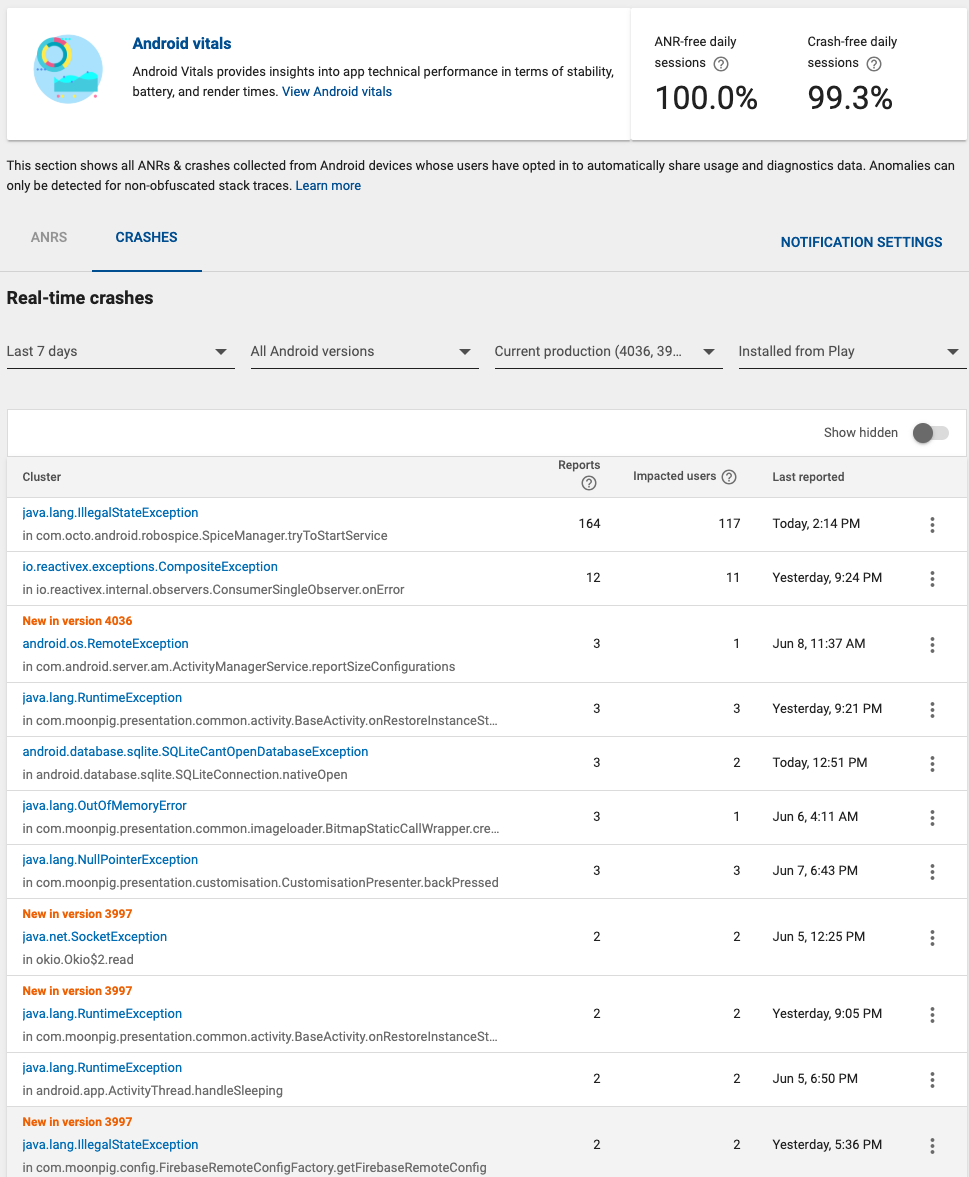
\includegraphics[width=13cm]{images/android-vitals-screenshots/moonpig/real-time-crashes-Screenshot-2019-06-10-at-15.42.34.png}
    \caption{Android Vitals: Moonpig snapshot of top crashes \nth{10} June 2019}
    \label{fig:av-moonpig-top-real-time-crashes-10-jun-2019}
\end{figure}

In Figure~\ref{fig:av-moonpig-top-real-time-crashes-10-jun-2019} Android Vitals shows the most frequent crash clusters for the production releases of the Moonpig Android app. The majority of crashes were an \texttt{IllegalStateException} in a third-party library SpiceManager, part of the RoboSpice opensource project https://github.com/stephanenicolas/robospice . 

This crash is an excellent example of how changes and new developments in the ecosystem can render what was reliable working software into software that is no longer fit for purpose, \emph{i.e.} RoboSpice was developed in 2012 to help developers simplify coding of asynchronous networking requests https://github.com/stephanenicolas/robospice and the library worked really well at the time and for several years afterwards. It became popular as a result and was used widely by many teams, including at Moonpig. However, as the Google Android platform morphed some of the changes to Android were incompatible with RoboSpice. And with Android Oreo (Release 8.0) changes to the way background services worked broke the functionality of the library sufficiently that the project was archived by the creator and project owner https://github.com/stephanenicolas/robospice/issues/467 

For apps that used RoboSpice the crash rate increased on the newer releases of Android, for example Figure~\ref{fig:av-moonpig-crash-rate-groupings} shows the crash rates by Android version were lowest on Android 7, higher for Android 8 and 8.1, and significantly higher again for Android 9. The teams needed to allocate time and energy to finding a suitable alternative to RoboSpice and then implement and test the new approach. Android Vitals helped provide an indication of the effects of the crashed and therefore provided evidence the development team could use to assess and prioritise the work.

\begin{figure}
    \centering
    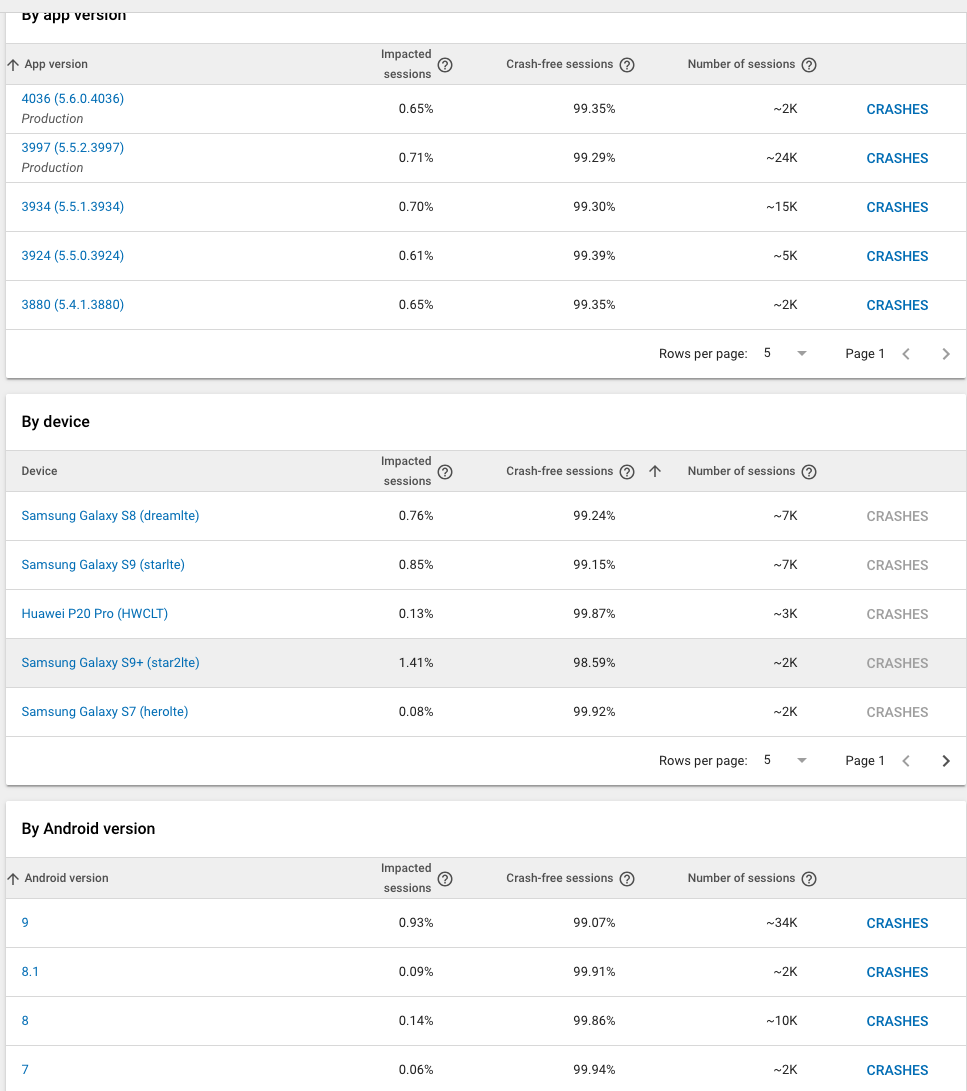
\includegraphics[width=13cm]{images/android-vitals-screenshots/moonpig/Screenshot 2019-06-10 at 15.41.23.png}
    \caption{Android Vitals: Moonpig various groupings of the crash rate \nth{10} June 2019}
    \label{fig:av-moonpig-crash-rate-groupings}
\end{figure}

\subsection{Moodspace}
Moodspace is an Android app aimed at improving mental health through various exercises incorporated into the app. It was released in 2019, with over 150K downloads by early 2020~\citep{objectbox2020_moodspace_interview}. Ian Alexander, the interviewee, was the software developer, co-founder, and runner of the company~\citep{objectbox2020_moodspace_interview} so he combines technical and operational responsibilities. He is an experienced app developer and also trained as a chemical engineer.  % https://www.linkedin.com/in/ian-alexander-01353340/

(\nth{13} June 2019)
% Source https://mail.google.com/mail/u/0/?q=kiwix+crash+rate+#search/kiwix+crash+rate/KtbxLzGHgCVznXxsGDjVgJGLFwmmGXxvxq
I love Android vitals - especially \textbf{core vitals}. Seeing your app in comparison to apps of peers provides some great motivation to step up your game. The only issue I have with core vitals is that I can't see them all! We are by no means a big app, so don't have enough data to meet googles standard for anonymised results, so results for most of the core vitals are hidden. I don't quite understand why this should be the case as the headline figure of your apps performance surely doesn't have to rely on anonymous data? Whereas the drilled down details of a core vital should be anonymous, so maybe the details view could just be blocked instead of hiding the entire core vital? To give context, MoodSpace has at least 4k monthly users, so there must be plenty of apps which get little or no use form core vitals, simply from them being hidden.

As for the other tools Google provides:
\begin{itemize}
    \item \textbf{ANR \& crashes} - I usually use crashlytics, so never really use this tab. the reason being, that the play console used to be very unreliable for crashes. But by the looks of it, it seems to have improved a lot, and pretty much matches the crashes I see in crashlytics now. Looking at it now, I actually noticed an ANR which could probably be fixed!
    \item \textbf{Pre launch reports} - I don't usually use this. Although this tool provides a nice safety net, it's quite basic, so any bugs that would cause the pre launch tests to fail have been found pre uploading through some quick manual testing. I actually ended up ignoring most pre launch reports when accessibility problems used to trigger failures, as we don't really have the resources to handle accessibility for now. But this seems to have changed in the last few months and accessibility problems don't cause a host of errors - maybe a way to ignore issues would be useful? In fact, pre-launch reports currently don't run on my app and fail with an incompatible apk error, not too sure why thats the case...
    \item \textbf{App signing} - very useful! and always use this since it was added.
    \item \textbf{Seperate release tracks} - love them! Especially since the addition of the internal track. The only issue was that I couldn't easily distribute debug versions of the app from the play store, and had to use a 3rd party tool to achieve that. Although Google have recently added Internal app sharing which should remedy that problem - however, I haven't figured out how to integrate that into our continuous integration process quite yet.
    \item \textbf{App bundles} - I'm still trying to integrate this, but as our new apps going to be heavily illustrated, this should cut our apk size significantly
\end{itemize}

As for several things I think are missing:

\begin{itemize}
    \item A gradle plugin to integrate play store uploading into CI processes. I currently use a 3rd party plugin to do this, but it would feel a little more secure if it came from Google.
    \item Top line core vitals figures even if you don't have enough users!
    \item Someway for testers to download old apks from either internal app sharing, or the internal release track.
\end{itemize}

I've attached the ANR and crash rates for the app. As I say, I usually use Firebase crashlytics, so don't really fix crash issues from Play store data.

You're welcome to use any data or comments in your research! If you do use it, please send over a copy.

(\nth{15} June 2019)
I think there's two things which has helped keep the app quite stable:
\begin{itemize}
    \item The app has the benefit that it's been around for quite a while without any major features being added. So most updates have been small and incremental, which has gradually increased it's stability. (This may change when the new, big update drops...)
    \item The app doesn't use any api, so all datas stored in very fast ORM databases like object-box (and uses memory caching). This enables the app to be mostly synchronous, which hugely cuts down on complexity of code. i.e. no need to handle loading, errors, or concurrency. This is a bit benefit! And cuts down on errors significantly, with no real impact on performance for users. To illustrate that it has little impact on users, I use firebase performance to run a trace on some methods that call the ORM/cache - it's peak duration is 40ms while the majority of calls take 3-6 ms.
\end{itemize} 

Crashlytics only covers the crash report of Android vitals, so unfortunately there's no way to get things like battery usage of ANR reports unless Google makes those reports available :(. In terms of crashes, I'd always prefer Crashlytics to Android vitals, simply because there are added features like non-fatal reporting and logs which can make surfacing the cause of errors much easier (but do take need added effort to integrate compared to android vitals).

There's been a change of branding of the app development organisation to \href{https://play.google.com/store/apps/developer?id=Chachi+Productions&hl=en_GB&gl=US}{Chachi Productions}. \url{https://www.appbrain.com/dev/Chachi+Productions/}


\newthought{Notes to integrate into the case study}
\begin{itemize}
    \item \url{https://www.psycom.net/25-best-mental-health-apps} Helps set the context for these apps.
    \item \url{https://objectbox.io/moodspace-mobile-app-use-case/} An interview with the founder Ian Alexander on the technological choices, particularly objectbox as the database. He'd mentioned the performance was lightning fast and one reason the app was performant and reliable. 
    \item ``Built MoodSpace, a digital platform empowering everyone to take control of their mental health. MoodSpace began as a side project which later took on a round of funding and with a team of 6 supported a user base of 300k. Although no longer pursued as a business we continue to maintain the project and release regular updates to 10s of thousands of active users. The most recent iteration of the app was built with Kotlin, clean architecture, MVVM, Data binding, Gitlab CI, Coroutines/Flow, and ObjectBox and was architected to enable the use of Kotlin Multiplatform to share ~60\% of the codebase between platforms."~\url{https://www.linkedin.com/in/ian-alexander-01353340/}
    \item 4.18/5.00 User Experience rating \url{https://onemindpsyberguide.org/apps/moodspace/}
    \item ``To make the app work well at all we collect the following anonymous data:
    \begin{itemize}
        \item Crash reports: If you've never seen the app crashing, it's because as soon as one happens, we get a crash report. A little red light flashes in our office, a loud siren blares, and we release a fix right away. It's quite annoying actually.
        \item Analytics: We assume you're going to use the app a certain way. We're almost always wrong, and you often surprise us. Analytics lets us see how people like you actually use the app, so we can make improvements to the right places. Analytics can use the Google Advertising ID to identify you. This doesn't tell us anything about you (it's just some numbers and letters), but if you really want to trick us you can reset your Google Advertising ID at any time. Go to your device Settings > Google > Ads."
    \end{itemize}~\citep{moodspace2021_privacy_policy}
\end{itemize}


\subsection{Local Halo}
MUST-DO complete this sub-section on Local Halo.

\begin{table}[htbp!]
    \centering
    \small
    \begin{tabular}{ll}
       Question &Answer  \\
       Website &\url{https://www.localhalo.com/} \\
       Founded &2018\\
       Business Domain &Digital neighbourhood groups in UK.\\
       Business type &Startup \\
       Technologies  &React Native \\
       Analytics Available &Sentry, Mixpanel, Google Play Console \\
       Development Practices &Cross-platform development
    \end{tabular}
    \caption{Case Study Overview: Localhalo}
    \label{tab:local_halo_anaytics_overview}
\end{table}

\subsubsection{Experiences of using mobile analytics}
Localhalo incorporate two analytics libraries into their cross-platform mobile application: sentry for crash reporting and mixpanel for business-oriented usage analytics. For their Android app they also have access to Google Play Console.

They experience numerous crashes reported by Sentry, which occur within the React Native runtime environment. Sentry provides email alerts to the development team together with summary reports, (Figure~\ref{fig:localhalo-sentry-weekly-report-21-sep-2020} is example for the period~\nth{14} to~\nth{21} September 2020), and online access to their analytics.

A release in March 2020 had a high crash rate for the production release of their Android app. The top crash cluster was for:

\texttt{java.lang.RuntimeExceptionhost.exp.exponent.experience.a\$b.run}. 

This was traced to a problem in the expo library they used in the app~\url{https://github.com/expo/expo/issues/5839}. In that issue several developers for different Android apps provide data from Google Play Console confirming they also receive similar crash clusters. The cause has not yet been definitively traced or addressed, however for the LocalHalo app the crashes stopped being reported once a new release of the Android app, release 1.3.0, was released around \nth{6} April 2020.

\begin{figure}[htbp!]
    \centering
    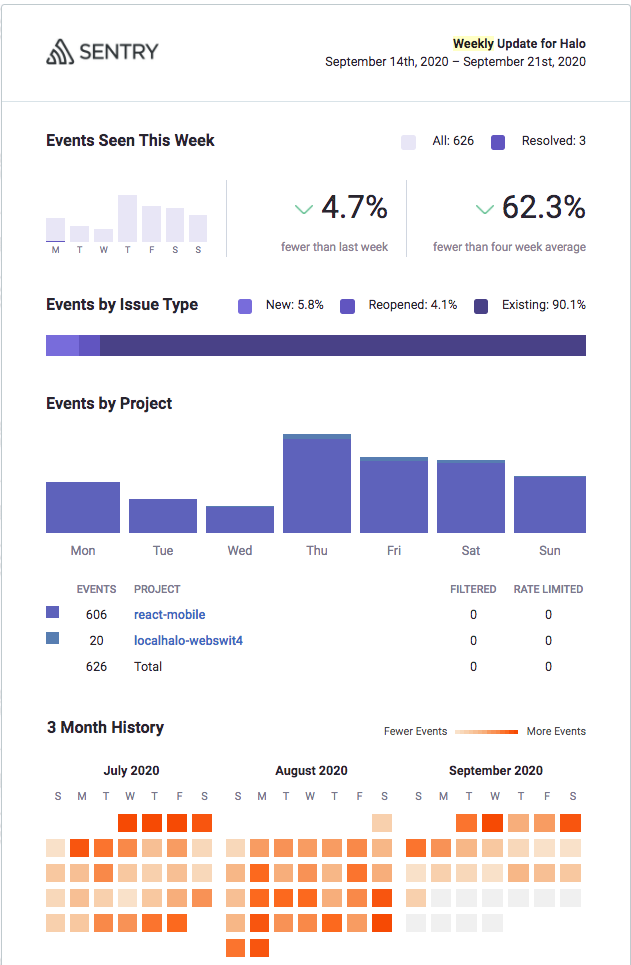
\includegraphics[width=9cm]{images/localhalo/sentry-weekly-report-21-Sep-2020.png}
    \caption{LocalHalo: Sentry weekly report 14 - 21 September 2020}
    \label{fig:localhalo-sentry-weekly-report-21-sep-2020}
\end{figure}

\textbf{Sentry}

MUST-DO Check in Sentry for the various types of error. How actively are the development team reading, reviewing and addressing crashes being reported? 

\begin{figure}[htbp!]
\centering
\begin{minipage}{.5\textwidth}
  \centering
  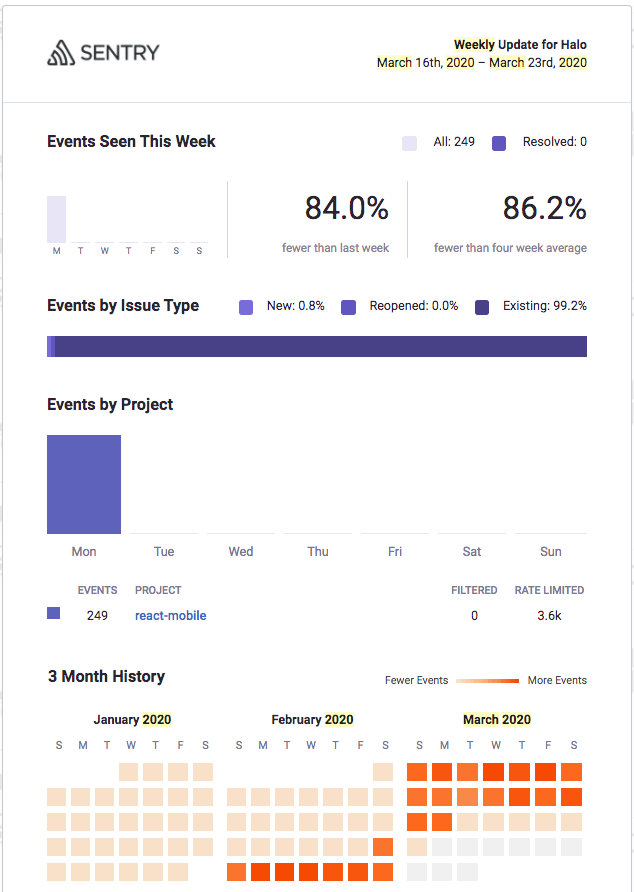
\includegraphics[width=.8\linewidth]{images/localhalo/sentry-weekly-report-16-mar-2020.png}
  \captionof*{figure}{\nth{16} -~\nth{22} March 2020}
  \label{fig:localhalo-sentry-weekly-report-16-mar-2020}
\end{minipage}%
\begin{minipage}{.5\textwidth}
  \centering
  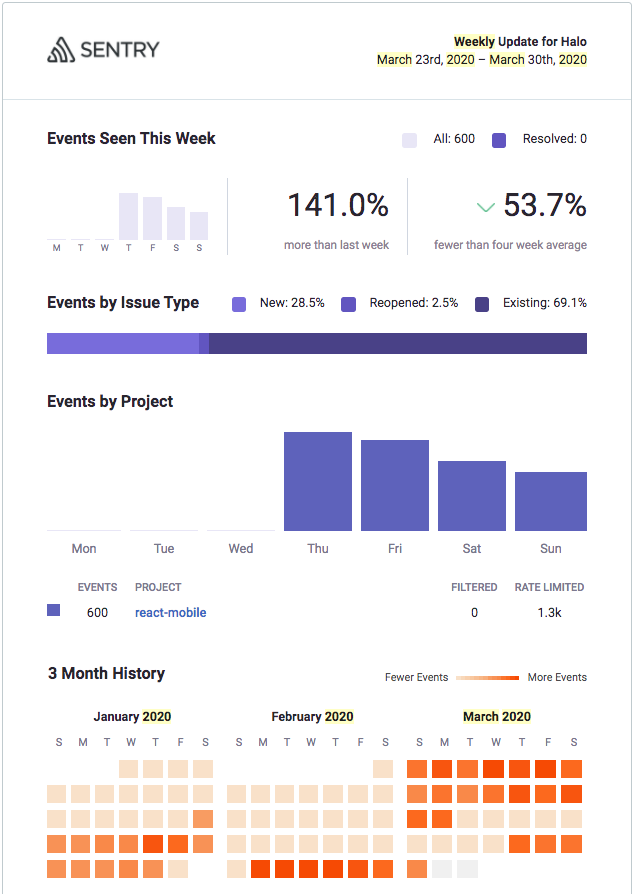
\includegraphics[width=.8\linewidth]{images/localhalo/sentry-weekly-report-23-mar-2020.png}
  \captionof*{figure}{\nth{23} -~\nth{29} March 2020}
  \label{fig:localhalo-sentry-weekly-report-23-mar-2020}
\end{minipage}
    \caption{Missing data reported in Sentry}
    \label{fig:sentry-missing-data-march-2020}
\end{figure}

\begin{comment}


\begin{figure}[htbp!]
    \centering
    %\subfigure[]{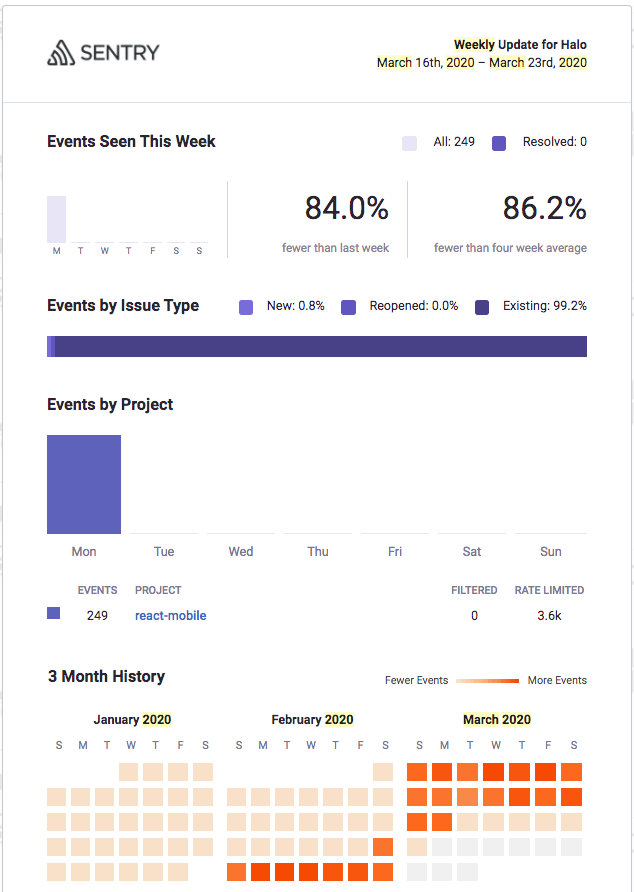
\includegraphics[width=0.4\textwidth]{images/localhalo/sentry-weekly-report-16-mar-2020.png}\caption{\nth{16} -~\nth{22} March 2020}\label{localhalo-sentry-weekly-report-16-mar-2020}}
    \subfigure[]{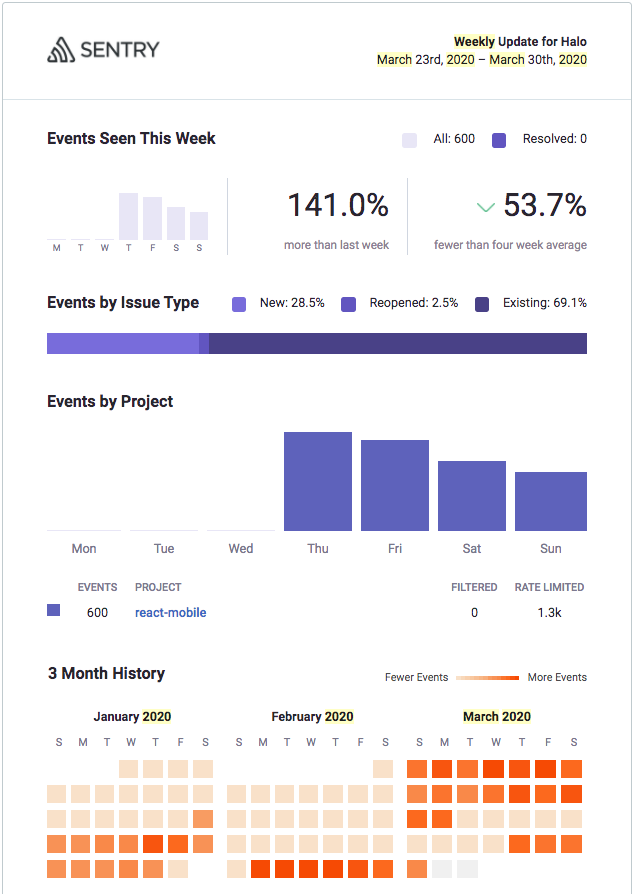
\includegraphics[width=0.4\textwidth]{images/localhalo/sentry-weekly-report-23-mar-2020.png}%\caption{\nth{23} -~\nth{29} March 2020}%\label{localhalo-sentry-weekly-report-23-mar-2020}
    }
    \caption{Missing data reported in Sentry}
    \label{fig:sentry-missing-data-march-2020}
\end{figure}
\end{comment}

%TODO fix the layout of the above figures: try: https://tex.stackexchange.com/questions/37581/latex-figures-side-by-side/37597#37597
Data missing from reports from~\nth{17} March to~\nth{25} March 2020 which affected the statistics around the time of the crashes related to Expo. Figure~\ref{fig:sentry-missing-data-march-2020} illustrates the gap across the two weekly reports. 

SHOULD-DO Consider summarising the crash totals per week. 

\textbf{MUST-DO} write up what we learn from the localhalo case study. external libraries can adversely affect the reliability of apps. Even small development teams can and do use multiple mobile analytics libraries. What can developers learn from the various reports provided by Sentry? How does cross-platform development in react-native affect the app reliability? are there crashes that only occur on Android or iOS? What's the correlation between crashes reported in Android Vitals and Sentry?


\subsection{Summary of Field Reports}
Active and ongoing use. 

%%% Ad-hoc notes from meeting Jakob D. Moonpig
% Business changes including the company's IPO mean the company has cut back on information they're willing to share internally and externally (e.g. for my PhD research).

\newpage

\section{A major corporation case study}

\textbf{Context} Acceptable use of PII. Fast growth of the team and very rapid initial growth of use of the service. High crash rates led to abandonment by users. 

\textbf{Relevance}
A wealthy corporation with large engineering teams can choose from any of the commercial mobile analytics tools and/or develop their own. They need to deliver software at scale and that scales. They have far larger professional software development teams than any of the other case-studies and face different challenges. They already use multiple mobile analytics tools, their challenge is to harness them consistently and productively to improve the `health' of their software and service to help staunch their loss of users because of software failures. In parallel they aim to launch new features that need to work for millions of users and serve both business-to-business and business-to-consumer users.

% A major corporation with millions of paying customers launch a free service in their main territory. Take up is rapid. 

\subsection{Methodology}
Consultant and advisor to the team with access to the key commercial sources of client-side analytics and access to the source code of the Android app and related library project.

\textbf{Priorities} data pipelines, ability to query across the many data sources without silos, 

\textbf{Some example issues} multiple analytics tools and data sources incorporated into the software and services, and yet extremely high ANR rates, very high crash rates. DNS error, how the error was discovered. 

\subsection{Lessons learned and/or confirmed}
Not all users of clients update, and a buggy release may leave a large stain on the statistics for the app. As the development team size increases so does the tendency to entropy in the implementation and use of embedded analytics. Furthermore, the team need to consistently check and apply the results of the many and various analytics services if they are to manage and improve the reliability and performance of their software.

The tools need to scale to billions of events per day.

Android Vitals provides a unique source of information, on ANR errors. Microsoft Windows does not offer equivalent reporting to the app developers. %TBD what Apple provides.

Blind spots exist, as do inconsistencies in the various end-to-end data collection and reporting in each analytics offering. 


\newpage


\section{Research in logging practices}
Early research explored ways developers of opensource Android apps use local logging, a complementary and oft used approach intended to help developers learn more about how their app behaves locally at run-time. 

\begin{itemize}
    \item Our research.
    \item The opensource tools we created to facilitate the testing and analysis of logging by Android developers.
    \item Explorations in methods to improve the effectiveness of logging and the analysis of log messages generated by apps.
\end{itemize}

\subsection{Designing logging}
Unstructured logging can serve immediate needs, for instance to trace code execution or display the value of a variable at run-time. The resulting entries into a log file have limited value in terms of longer term analysis and they may also be harder to identify, filter, and lack relevant content for such analysis.

In the domain of logging both business and research consider logging design important and valuable. 

Implementation choices: 

\subsection{Testing logging}
TBC



\newpage

\section{A tools provider's perspective: Iterative.ly}
\label{section-tool-providers-perspective}
The use of mobile analytics extends beyond the development role in a team or organisation. Software tools should also serve the project rather than being the master of it. ~\citep{budgen1993_case_tools_masters_or_servants} raises a similar issue of whether CASE tools are masters or servants. There is a significant risk that development teams lose control of the data, and/or are constrained by the policies, implementation, and so on of a particular tool provider. Companies including Iteratively, Avo, and Segment aim to provide aspects of: freedom of choice and the ability to choose, cross team alignment and visibility of the use of embedded (in-app) analytics, and compliance. Here, Iteratively is included as a mini case-study of what one of these companies is doing to help development teams in their use of embedded (in-app) mobile analytics.

%Cross team tracking and alignment on the use of embedded (in-app) mobile analytics 

%Introduce the company: location, age, type of business, etc. Information freely given with permission to use it generally, including for research purposes.
Iteratively was founded on \nth{20} February 2019 and based in Seattle, Washington State, USA by two experienced co-founders. They contacted me in May 2020 as they were interested in my perspective and research into mobile analytics. %Sources include: https://iterative.ly/about/ https://www.crunchbase.com/organization/iteratively
%
Subsequently, they kindly agreed to contribute to this research as a small case study of a startup aiming to develop products to help development teams improve their use of mobile analytics. They provided all information is freely given with permission to use it generally, including for research purposes.

This research case study include these research methods: semi-structured interviews, a walk-through of the tools and service, collaborative verbal discussions and various written materials.

Their service is self-described as ``GitHub for your analytics", providing a versioned schema registry for analytics events~\footnote{Source: a non-public document used with permission.}.
%
Their value proposition: a versioned schema for web and mobile analytics. Tools that generate the client-side SDK that developers then include in their apps. They use lint tools to verify that events have been instrumented correctly. At runtime their SDK validates event payloads match the schema to help enforce data quality. They provide tools that help detect some forms of PII with the aim of helping improve legal compliance.  

Relevance to the research in the thesis: tools to help design and validate the analytics content. A whitebox insight into an analytics provider who also develop and provide tools to help organisations improve their use of mobile and web analytics. 


\subsection{Related work}
- Mention similar work avo.app
- segment.io - indicates the growth and relevance of mobile analytics as a market, of addressing data ownership and freedom of choice of analytics implementations. 

\subsection{Their market research}
MUST-DO expand this section, mainly to cover key points in their early market research and the relevance to the research in this thesis.

What leading edge businesses value in their analytics tools? (10 dots voting examples, see Figure~\ref{tab:10dots_voting_iteratively}), their early market research (see the first notion.io document.)


Dot voting is a simple voting exercise where each participant has a finite number of dots they can vote with to prioritise a set of choices~\citep{18f_dot_voting}. Dot voting is used in many software development teams who use Agile software development practices, and offers easy and lightweight voting of ideas~\citep{nngroup_dot_voting}. There are criticisms of the technique, for instance where poorly designed options split votes, where people vote tactically, or where people appropriate and use dots from others~\citep{dotmocracy}. The approach used by iteratively mitigates against these concerns through the design and implementation of the voting. 

Iteratively's method uses a video call with screen sharing. Each participant has already agreed to take part in the research exercise which includes the ten dots voting as part of a semi-structured interview. They are presented with the prepared template `Spend 10 coins', as illustrated in Figure~\ref{fig:iteratively-spend-10-dots}. The interviewer explains each item in order until each of them have been explained. Some interviewees allocate the coins (dots) early others wait until the end of the explanation.


\begin{figure}[htbp!]
    \centering
    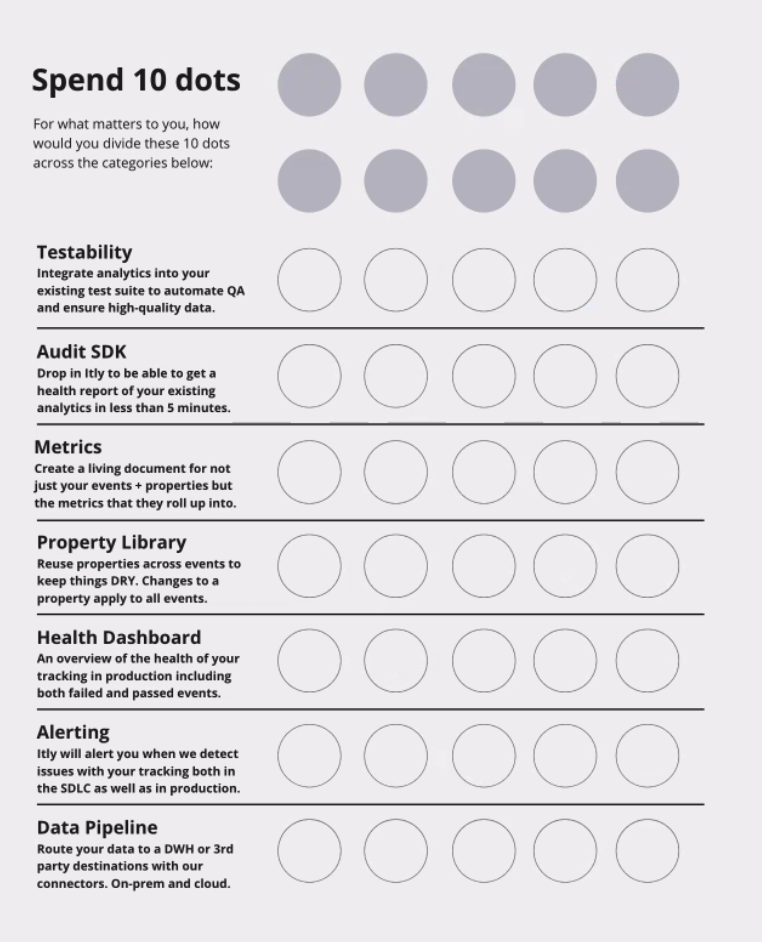
\includegraphics[width=10cm]{images/iteratively/spend-10-dots.png}
    \caption{Interatively spend 10 dots}
    \label{fig:iteratively-spend-10-dots}
\end{figure}

According to Iteratively the votes are helpful, and the discussions around the topics more so.  Figure~\ref{fig:iteratively-dot-voting-example} is an example where the votes have been cast. 

\begin{figure}[htbp!]
    \centering
    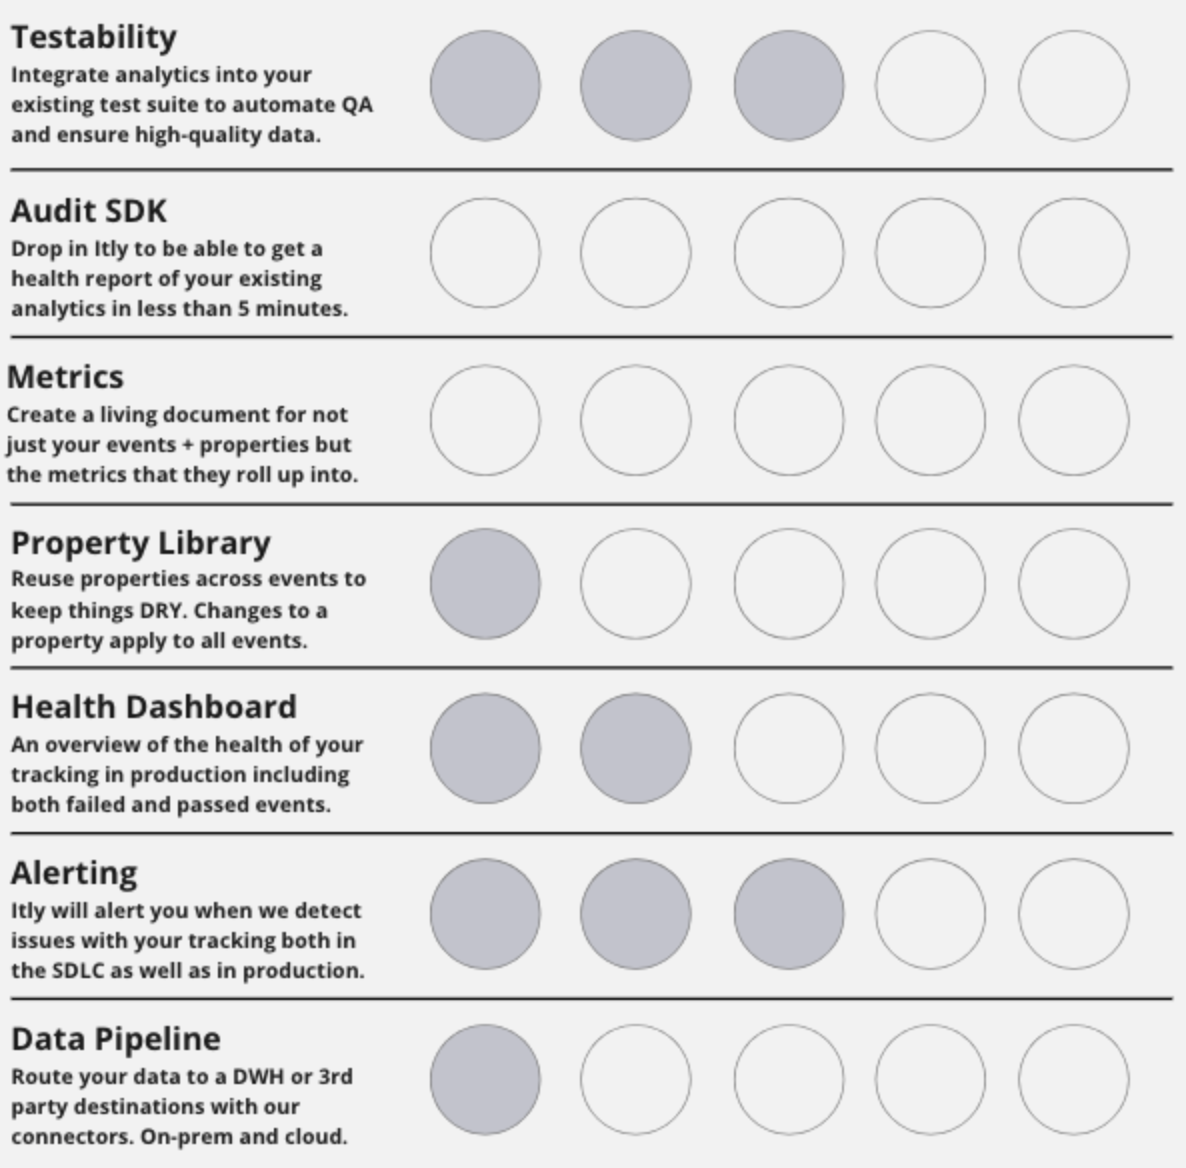
\includegraphics[width=10cm]{images/iteratively/dot-voting-example.png}
    \caption{Iteratively dot voting example}
    \label{fig:iteratively-dot-voting-example}
\end{figure}


Seven candidate topics were used, here are the exact wordings of each topic description:
\begin{enumerate}
    \item \textbf{Testability}: Integrate analytics into your existing test suite to automate QA and ensure high-quality data.
    \item \textbf{Audit SDK}: Drop in itly\footnote{itly: Iteratively.} to be able to get a health report of your existing analytics in less than 5 minutes.
    \item \textbf{Metrics}: Create a living document for not just your events + properties but the metrics they roll up into.
    \item \textbf{Property Library}: Reuse properties across events to keep things DRY. Changes to a property apply to all events.
    \item \textbf{Health Dashboard}: An overview of the health of your tracking in production including both failed and passed events.
    \item \textbf{Alerting}: Itly will alert you when we detect issues with your tracking both in the SDLC\footnote{SDLC: Software Development Life Cycle.} as well as in production.
    \item \textbf{Data Pipeline}: Route your data to a DWH\footnote{DWH: Data Warehouse.} or 3rd party destinations with our connectors. On-prem~\footnote{On-prem: On premise.} and cloud.
\end{enumerate}
These topics were chosen to help Iteratively with planning their product roadmap. They also provide a useful context and perspective for the research into using mobile analytics from product and data engineering perspectives. With one exception, all the participants actively use analytics in their software and have expressed an interest in improving their approach into incorporating and using analytics in their apps.

\begin{table}[htbp!]
 
    \centering
    \small
    \setlength{\tabcolsep}{4pt} %% default is 6pt
    %% With thanks to http://tex.my/how-to-deal-with-wide-tables/ for the \tabcolsep tip
    \begin{tabular}{lr|rrrrrrrrrrrrrr}
    % SHOULD-DO Added column span over the participants, reduce the heavy lines on the table.
                     &Sum &A  &B  &C  &D  &E  &F  &G  &H  &I  &J &K &L &M &N\\
    \hline     
    Testability         &30 &3  &3  &3  &1  &   &3  &3  &1  &5  &3 &  &3 &1 &1\\
    Audit SDK           &25 &   &2  &   &   &2  &2  &3  &1  &2  &1 &3 &3 &5 &1\\
    Metrics             &6  &   &   &   &   &   &1  &   &   &   &  &  &1 &3 &1\\
    Property library    &21 &1  &3  &3  &2  &3  &2  &1  &   &   &1 &1 &1 &  &3\\
    Health Dashboard    &17 &2  &   &2  &   &3  &   &2  &2  &   &2 &2 &  &1 &1\\
    Alerting            &18 &3  &2  &   &2  &   &2  &   &4  &   &3 &  &1 &  &1\\
    Data Pipeline       &18 &1  &   &2  &   &2  &   &1  &2  &3  &  &4 &1 &  &2\\
         
    \end{tabular}
    \caption{10 dots voting Iteratively market research}
    \label{tab:10dots_voting_iteratively}

\end{table}
% My spreadsheet https://docs.google.com/spreadsheets/d/1Acti8klc6JvLu_NAR7t7cC8XdMHx-FIkfSHcqt_srwc/edit#gid=0 
% Source from iterative.ly's miro board https://miro.com/app/board/o9J_kujB-Y4=/ 

The first ten sets of dot votes rank the choices as follows: Testability (25), Property Library (16), Alerting (16), Audit SDK (13), Health Dashboard (13), Data Pipeline (11), and lastly Metrics (1). The next three sets of dot votes cement testability as the \#1 ranking, they also bump up auditing the use of the SDK to second place in the rankings, and even metrics gets a boost to 5 votes in total. 

With 14 sets of votes, the ranking is still volatile and the scores unlikely to be sufficiently robust to depend on. Nonetheless several indications are starting to emerge. 
These votes indicate testability is the most desired property for designing and implementing analytics where the analytics can help shape and drive automated testing of software based on production usage characteristics. Auditing of the SDK is in a strong second place, to provide an immediate health check of the existing analytics. Participants who use Iteratively's services score property library highly as they have experienced the value in this capability. Alerting when issues are detected with the tracking in the SDLC and production ties in joint fourth place with the data pipeline. Data pipeline is more important than it may appear, as some of the respondents professed they preferred alternatives to using Iteratively to provide the data pipeline. The interviews indicated that data pipelines are more important than the score indicates.

The seven topics were chosen quickly and not necessarily intended to be comprehensive. One omission we discussed is the area that encompasses: privacy, Personally Identifiable Information (PII), and compliance, nonetheless these are believed to be important to Iteratively's current and potential customers and an area they are actively working on.

\subsection{Evaluation of their service}
SHOULD-DO apply their tooling for an Android app for an existing app and discuss the effects of using their tooling and service. % Possibly do this with Joe Reeve to include his perspective as he transitions from outsider to insider at the company?

\subsection{Indications of where mobile analytics is heading}
Iteratively and several companies with similar value propositions indicate several potential trends in the use of mobile analytics. These trends include: mobile analytics is now subject to quality criteria, where organisations seek mechanisms to help them integrate mobile analytics as a first-class citizen in app development, potentially at least as valuable as some features in their apps. Also there is a need and a desire to use and manage mobile analytics effectively, including ownership and management of the data that is collected by the many and various mobile analytics tools. 


\newpage

\section{Summary of Case Studies}
MUST-DO revise and update this summary close to submitting the thesis - when the main canon of the work is closed; i.e. when there are no new case studies likely to be added.

The case studies includes a useful range of Android apps developed by independent teams using a variety of programming languages, mindsets, objectives, and constraints. In each team they learned to actively focus on stability metrics as reported in various technology-facing analytics tools, and the developers continue to see the merit of doing so on an ongoing basis.